\documentclass[12pt,a4paper,parskip=full]{scrartcl}
\KOMAoption{bibliography}{totoc}
\KOMAoption{listof}{totoc}

%display boundaries
%\usepackage{showframe}

\usepackage{cite}
\usepackage[pdftex]{graphicx}
\graphicspath{{graphics/}}

\usepackage[cmex10]{amsmath}
\usepackage{amssymb}
\usepackage{gensymb}
\usepackage{listings}
\usepackage{tocloft}
\usepackage{subcaption}

\usepackage{url}

\usepackage{makeidx}
\usepackage[colorlinks,hyperindex,plainpages=false,
pdftitle={High-frequency characterization of a Software Defined Radio (SDR) platform},
pdfauthor={Gernot Vormayr},
pdfsubject={Bachelor thesis},
pdfkeywords={Hochfrequenz,Software Defined Radio,SDR,GNU Radio,USRP},
pdfpagelabels,
pagebackref,
bookmarksopen=false
]{hyperref}

\usepackage[binary-units]{siunitx}
\usepackage{pgfplots}

\pgfplotsset{compat=1.11}
\pgfplotsset{every axis plot/.append style={smooth},every axis/.append style={grid=major,legend style={font=\footnotesize}}} 

\usepgfplotslibrary{units}
\pgfplotsset{unit code/.code 2 args={\si{#1#2}}}

\usepackage{tikz}
\usetikzlibrary{dsp,chains,fit,matrix,positioning,scopes,calc,backgrounds,arrows,decorations.pathmorphing,shapes.misc}
\usepackage{circuitikz}

\makeatletter

\ctikzset{rf/width/.initial=0.75}
\ctikzset{rf/height/.initial=0.75}
\ctikzset{rf/filter/sinewidth/.initial=0.8}
\ctikzset{rf/filter/sineheight/.initial=0.2}
\ctikzset{rf/switch/length/.initial=0.6}
\ctikzset{rf/adc/width/.initial=1}


\long\def\pgfrfdeclarenode#1#2#3{
    \pgfdeclareshape{#1}
    {
        \anchor{center}{
            \pgfpointorigin
        }
        \savedanchor\northwest{%
            \pgf@y=\pgfkeysvalueof{/tikz/circuitikz/bipoles/length}
            \pgf@y=\pgfkeysvalueof{/tikz/circuitikz/rf/height}\pgf@y
            \pgf@y=.5\pgf@y
            \pgf@x=\pgfkeysvalueof{/tikz/circuitikz/bipoles/length}
            \pgf@x=.5\pgf@x
            \pgf@x=-\pgfkeysvalueof{/tikz/circuitikz/rf/width}\pgf@x
        }
        \anchor{north}{
            \northwest
            \pgf@x=0pt
        }
        \anchor{south}{
            \northwest
            \pgf@x=0pt
            \pgf@y=-\pgf@y
        }
        \anchor{west}{
            \northwest
            \pgf@y=0pt
        }
        \anchor{east}{
            \northwest
            \pgf@y=0pt
            \pgf@x=-\pgf@x
        }
        \anchor{south west}{
            \northwest
            \pgf@y=-\pgf@y
        }
        \anchor{north east}{
            \northwest
            \pgf@x=-\pgf@x
        }
        \anchor{north west}{
            \northwest
        }
        \anchor{south east}{
            \northwest
            \pgf@x=-\pgf@x
            \pgf@y=-\pgf@y
        }	  
        \anchor{base}{
            \northwest
            \pgf@x=0pt	  	
        }
        \anchorborder{
            \@tempdima=\pgf@x
            \@tempdimb=\pgf@y
            \northwest
            \pgf@xa=-\pgf@x
            \pgf@ya=\pgf@y
            \pgfpointborderrectangle{\pgfpoint{\@tempdima}{\@tempdimb}}{\pgfpoint{\pgf@xa}{\pgf@ya}}
        }
        #3
        \backgroundpath{			
            \pgfsetcolor{\pgfkeysvalueof{/tikz/circuitikz/color}}	

            \northwest
            \pgf@circ@res@up = \pgf@y 
            \pgf@circ@res@down = -\pgf@y
            \pgf@circ@res@right = -\pgf@x
            \pgf@circ@res@left = \pgf@x

            \pgfscope
                \pgfsetcornersarced{\pgfpoint{4pt}{4pt}}
                \pgfpathrectanglecorners{\pgfpoint{\pgf@circ@res@left}{\pgf@circ@res@down}}{\pgfpoint{\pgf@circ@res@right}{\pgf@circ@res@up}}
                \pgfstroke
            \endpgfscope

            #2

        }
    }
}

\long\def\pgfrfdeclaremonopole#1#2{
    \pgfrfdeclarenode{#1}{#2}{
        \anchor{A}{
            \northwest
            \pgf@y=0pt
        }
    }
}

\long\def\pgfrfdeclarebipole#1#2{
    \pgfrfdeclarenode{#1}{#2}{
        \anchor{A}{
            \northwest
            \pgf@y=0pt
        }
        \anchor{B}{
            \northwest
            \pgf@y=0pt
            \pgf@x=-\pgf@x
        }
    }
}

\long\def\pgfrfdeclaretripole#1#2{
    \pgfrfdeclarenode{#1}{#2}{
        \anchor{A1}{
            \northwest
            \pgf@y=0pt
        }
        \anchor{B1}{
            \northwest
            \pgf@y=0.5\pgf@y
            \pgf@x=-\pgf@x
        }
        \anchor{B2}{
            \northwest
            \pgf@y=-0.5\pgf@y
            \pgf@x=-\pgf@x
        }
    }
}

\long\def\pgfrfdeclarequadpole#1#2{
    \pgfrfdeclarenode{#1}{#2}{
        \anchor{A1}{
            \northwest
            \pgf@y=0.5\pgf@y
        }
        \anchor{A2}{
            \northwest
            \pgf@y=-0.5\pgf@y
        }
        \anchor{B1}{
            \northwest
            \pgf@y=0.5\pgf@y
            \pgf@x=-\pgf@x
        }
        \anchor{B2}{
            \northwest
            \pgf@y=-0.5\pgf@y
            \pgf@x=-\pgf@x
        }
    }
}

\long\def\pgfrfdeclaredadc#1#2{
    \pgfdeclareshape{#1}
    {
        \anchor{center}{
            \pgfpointorigin
        }
        \savedanchor\northwest{%
            \pgf@y=\pgfkeysvalueof{/tikz/circuitikz/bipoles/length}
            \pgf@y=\pgfkeysvalueof{/tikz/circuitikz/rf/height}\pgf@y
            \pgf@y=.5\pgf@y
            \pgf@x=\pgfkeysvalueof{/tikz/circuitikz/bipoles/length}
            \pgf@x=.5\pgf@x
            \pgf@x=-\pgfkeysvalueof{/tikz/circuitikz/rf/adc/width}\pgf@x
        }
        \anchor{north}{
            \northwest
            \pgf@x=0pt
        }
        \anchor{south}{
            \northwest
            \pgf@x=0pt
            \pgf@y=-\pgf@y
        }
        \anchor{west}{
            \northwest
            \pgf@y=0pt
        }
        \anchor{east}{
            \northwest
            \pgf@y=0pt
            \pgf@x=-\pgf@x
        }
        \anchor{south west}{
            \northwest
            \pgf@y=-\pgf@y
        }
        \anchor{north east}{
            \northwest
            \pgf@x=-\pgf@x
        }
        \anchor{north west}{
            \northwest
        }
        \anchor{south east}{
            \northwest
            \pgf@x=-\pgf@x
            \pgf@y=-\pgf@y
        }	  
        \anchor{base}{
            \northwest
            \pgf@x=0pt	  	
        }
        \anchor{A}{
            \northwest
            \pgf@y=0pt
        }
        \anchor{B}{
            \northwest
            \pgf@y=0pt
            \pgf@x=-\pgf@x
        }
        \anchorborder{
            \@tempdima=\pgf@x
            \@tempdimb=\pgf@y
            \northwest
            \pgf@xa=-\pgf@x
            \pgf@ya=\pgf@y
            \pgfpointborderrectangle{\pgfpoint{\@tempdima}{\@tempdimb}}{\pgfpoint{\pgf@xa}{\pgf@ya}}
        }
        \backgroundpath{			
            \pgfsetcolor{\pgfkeysvalueof{/tikz/circuitikz/color}}	

            \northwest
            \pgf@circ@res@up = \pgf@y 
            \pgf@circ@res@down = -\pgf@y
            \pgf@circ@res@right = -\pgf@x
            \pgf@circ@res@left = \pgf@x

            #2

        }
    }
}

\pgfrfdeclarebipole{attenuator}{
    \pgfscope             
        \pgftransformscale{.5}
        \pgfnode{resistorshape}{center}{}{pgf@att}{\pgfusepath{stroke}}
    \endpgfscope
    \pgfpathmoveto{\pgfpoint{\pgf@circ@res@left}{0}}
    \pgfpathlineto{\pgfpointanchor{pgf@att}{b}}
    \pgfpathmoveto{\pgfpoint{\pgf@circ@res@right}{0}}
    \pgfpathlineto{\pgfpointanchor{pgf@att}{a}}
    \pgfusepath{draw}

}

\pgfrfdeclarebipole{vattenuator}{
    \pgfscope             
        \pgftransformscale{.5}
        \pgfnode{resistorshape}{center}{}{pgf@att}{\pgfusepath{stroke}}
    \endpgfscope
    \pgfpathmoveto{\pgfpoint{\pgf@circ@res@left}{0}}
    \pgfpathlineto{\pgfpointanchor{pgf@att}{b}}
    \pgfpathmoveto{\pgfpoint{\pgf@circ@res@right}{0}}
    \pgfpathlineto{\pgfpointanchor{pgf@att}{a}}
    \pgfusepath{draw}
    \pgfpathmoveto{\pgfpoint{0.5\pgf@circ@res@left}{0.7\pgf@circ@res@down}}
    \pgfpathlineto{\pgfpoint{0.5\pgf@circ@res@right}{0.7\pgf@circ@res@up}}
    \pgfsetarrowsend{stealth}
    \pgfusepath{draw}
}

\def\pgfrffiltersinewave{
        \pgfpathmoveto{\pgfpoint{\pgf@xb}{\pgf@yb}}
        \pgfpathsine{\pgfpoint{\pgf@xa}{\pgf@ya}}
        \pgfpathcosine{\pgfpoint{\pgf@xa}{-\pgf@ya}}
        \pgfpathsine{\pgfpoint{\pgf@xa}{-\pgf@ya}}
        \pgfpathcosine{\pgfpoint{\pgf@xa}{\pgf@ya}}
        \advance \pgf@yb by \pgf@circ@res@step
}

\long\def\pgfrfdeclarefilter#1#2{
    \pgfrfdeclarebipole{#1}{
        \pgfscope
            \pgf@yb = 0.5\pgf@circ@res@up
            \pgf@circ@res@step = -0.5\pgf@circ@res@up
            
            \pgf@xa = \ctikzvalof{rf/filter/sinewidth}\pgf@circ@res@right
            \divide \pgf@xa by 2
            \pgf@ya = \ctikzvalof{rf/filter/sineheight}\pgf@circ@res@up
            \pgf@xb = \ctikzvalof{rf/filter/sinewidth}\pgf@circ@res@left

            \pgfrffiltersinewave
            \pgfrffiltersinewave
            \pgfrffiltersinewave
            \pgfstroke
        \endpgfscope
        #2
    }
}

\def\pgfrfstrikewave#1{
    \pgf@ya = 0.5\pgf@circ@res@up
    \pgf@yb = #1\pgf@ya
    \advance \pgf@ya by -\pgf@yb
    \advance \pgf@ya by -2pt
    \pgfpathmoveto{\pgfpoint{-2pt}{\pgf@ya}}
    \advance \pgf@ya by 4pt
    \pgfpathlineto{\pgfpoint{2pt}{\pgf@ya}}
}

\pgfrfdeclarefilter{lowpass}{
    \pgfrfstrikewave{0}
    \pgfrfstrikewave{1}
    \pgfusepath{draw}
}

\pgfrfdeclarefilter{highpass}{
    \pgfrfstrikewave{1}
    \pgfrfstrikewave{2}
    \pgfusepath{draw}
}

\pgfrfdeclarefilter{bandpass}{
    \pgfrfstrikewave{0}
    \pgfrfstrikewave{2}
    \pgfusepath{draw}
}

\pgfrfdeclaretripole{altswitch}{
    \pgf@xa = \ctikzvalof{rf/switch/length}\pgf@circ@res@left
    \pgfpathmoveto{\pgfpoint{\pgf@circ@res@left}{0}}
    \pgfpathlineto{\pgfpoint{\pgf@xa}{0}}
    \pgfpathlineto{\pgfpoint{-\pgf@xa}{-0.5\pgf@circ@res@up}}
    \pgfpathlineto{\pgfpoint{\pgf@circ@res@right}{-0.5\pgf@circ@res@up}}
    \pgfpathmoveto{\pgfpoint{\pgf@circ@res@right}{0.5\pgf@circ@res@up}}
    \pgfpathlineto{\pgfpoint{-\pgf@xa}{0.5\pgf@circ@res@up}}
    \pgfusepath{draw}
    \pgfpathcircle{\pgfpoint{-\ctikzvalof{rf/switch/length}\pgf@circ@res@left}{-0.5\pgf@circ@res@up}}{1.5pt}
    \pgfusepath{draw,fill}
    \pgfsetfillcolor{white}
    \pgfpathcircle{\pgfpoint{-\ctikzvalof{rf/switch/length}\pgf@circ@res@left}{0.5\pgf@circ@res@up}}{1.5pt}
    \pgfusepath{draw,fill}
    \pgfpathmoveto{\pgfpoint{0}{0.25\pgf@circ@res@down}}
    \pgfmathsetmacro{\tikz@start@angle@temp}{(atan2(0.5*\the\pgf@circ@res@up,2*\ctikzvalof{rf/switch/length}*\the\pgf@circ@res@right))}
    \pgfpatharc{-\tikz@start@angle@temp}{+\tikz@start@angle@temp}{\ctikzvalof{rf/switch/length}\pgf@circ@res@right}
    \pgfsetarrowsend{stealth}
    \pgfusepath{draw}
}

\pgfrfdeclarequadpole{chswitch}{
    \pgf@xa = \ctikzvalof{rf/switch/length}\pgf@circ@res@left
    \pgfpathmoveto{\pgfpoint{\pgf@circ@res@left}{0.5\pgf@circ@res@up}}
    \pgfpathlineto{\pgfpoint{\pgf@circ@res@right}{0.5\pgf@circ@res@up}}
    \pgfpathmoveto{\pgfpoint{\pgf@circ@res@left}{0.5\pgf@circ@res@down}}
    \pgfpathlineto{\pgfpoint{\pgf@circ@res@right}{0.5\pgf@circ@res@down}}
    \pgfusepath{draw}
    \pgfpathmoveto{\pgfpoint{\ctikzvalof{rf/switch/length}\pgf@circ@res@left}{0.5\pgf@circ@res@up}}{1.5pt}
    \pgfpathlineto{\pgfpoint{\ctikzvalof{rf/switch/length}\pgf@circ@res@right}{0.5\pgf@circ@res@down}}{1.5pt}
    \pgfpathmoveto{\pgfpoint{\ctikzvalof{rf/switch/length}\pgf@circ@res@right}{0.5\pgf@circ@res@up}}{1.5pt}
    \pgfpathlineto{\pgfpoint{\ctikzvalof{rf/switch/length}\pgf@circ@res@left}{0.5\pgf@circ@res@down}}{1.5pt}
    \pgfsetdash{{3pt}{2pt}}{0pt}
    \pgfusepath{draw}
    \pgfsetfillcolor{white}
    \pgfsetdash{}{0pt}
    \pgfpathcircle{\pgfpoint{\ctikzvalof{rf/switch/length}\pgf@circ@res@left}{0.5\pgf@circ@res@up}}{1.5pt}
    \pgfpathcircle{\pgfpoint{\ctikzvalof{rf/switch/length}\pgf@circ@res@left}{0.5\pgf@circ@res@down}}{1.5pt}
    \pgfpathcircle{\pgfpoint{\ctikzvalof{rf/switch/length}\pgf@circ@res@right}{0.5\pgf@circ@res@up}}{1.5pt}
    \pgfpathcircle{\pgfpoint{\ctikzvalof{rf/switch/length}\pgf@circ@res@right}{0.5\pgf@circ@res@down}}{1.5pt}
    \pgfusepath{draw,fill}
}

\pgfrfdeclaredadc{adc}{
    \pgf@xa=\pgf@circ@res@left
    \divide \pgf@xa by 3
    \pgfpathmoveto{\pgfpoint{\pgf@circ@res@left}{0pt}}
    \pgfpathlineto{\pgfpoint{\pgf@xa}{\pgf@circ@res@up}}
    \pgfpathlineto{\pgfpoint{\pgf@circ@res@right}{\pgf@circ@res@up}}
    \pgfpathlineto{\pgfpoint{\pgf@circ@res@right}{\pgf@circ@res@down}}
    \pgfpathlineto{\pgfpoint{\pgf@xa}{\pgf@circ@res@down}}
    \pgfclosepath
    \pgfusepath{draw}
}

\pgfrfdeclaredadc{dac}{
    \pgf@xa=\pgf@circ@res@right
    \divide \pgf@xa by 3
    \pgfpathmoveto{\pgfpoint{\pgf@circ@res@right}{0pt}}
    \pgfpathlineto{\pgfpoint{\pgf@xa}{\pgf@circ@res@up}}
    \pgfpathlineto{\pgfpoint{\pgf@circ@res@left}{\pgf@circ@res@up}}
    \pgfpathlineto{\pgfpoint{\pgf@circ@res@left}{\pgf@circ@res@down}}
    \pgfpathlineto{\pgfpoint{\pgf@xa}{\pgf@circ@res@down}}
    \pgfclosepath
    \pgfusepath{draw}
}

\pgfrfdeclarebipole{amp}{
    \pgfscope             
        \pgftransformscale{.5}
        \pgfnode{buffer}{center}{}{pgf@amp}{\pgfusepath{stroke}}
    \endpgfscope
    \pgfpathmoveto{\pgfpoint{\pgf@circ@res@left}{0}}
    \pgfpathlineto{\pgfpointanchor{pgf@amp}{in}}
    \pgfpathmoveto{\pgfpoint{\pgf@circ@res@right}{0}}
    \pgfpathlineto{\pgfpointanchor{pgf@amp}{out}}
    \pgfusepath{draw}
}

\pgfrfdeclarenode{iqmix}{
    \pgfscope             
        \pgftransformshift{\pgfpoint{0.5\pgf@circ@res@right}{0.5\pgf@circ@res@up}}
        \pgftransformrotate{180}
        \pgftransformscale{.2}
        \pgfnode{mixer}{center}{}{pgf@mixi}{\pgfusepath{stroke}}
    \endpgfscope
    \pgfscope             
        \pgftransformshift{\pgfpoint{0}{0.5\pgf@circ@res@down}}
        \pgftransformrotate{180}
        \pgftransformscale{.2}
        \pgfnode{mixer}{center}{}{pgf@mixq}{\pgfusepath{stroke}}
    \endpgfscope
    \pgfscope             
        \pgftransformscale{.35}
        \pgfnode{rectangle}{center}{$90\degree$}{pgf@phase}{\pgfusepath{stroke}}
    \endpgfscope
    \pgfpathmoveto{\pgfpoint{\pgf@circ@res@left}{0pt}}
    \pgfpathlineto{\pgfpoint{0.6\pgf@circ@res@left}{0pt}}
    \pgfpathlineto{\pgfpoint{0.6\pgf@circ@res@left}{0.5\pgf@circ@res@up}}
    \pgfpathlineto{\pgfpointanchor{pgf@mixi}{out}}
    \pgfpathmoveto{\pgfpoint{0.6\pgf@circ@res@left}{0pt}}
    \pgfpathlineto{\pgfpoint{0.6\pgf@circ@res@left}{0.5\pgf@circ@res@down}}
    \pgfpathlineto{\pgfpointanchor{pgf@mixq}{out}}
    \pgfpathmoveto{\pgfpointanchor{pgf@mixi}{in}}
    \pgfpathlineto{\pgfpoint{\pgf@circ@res@right}{0.5\pgf@circ@res@up}}
    \pgfpathmoveto{\pgfpointanchor{pgf@mixq}{in}}
    \pgfpathlineto{\pgfpoint{\pgf@circ@res@right}{0.5\pgf@circ@res@down}}
    \pgfpathmoveto{\pgfpoint{0pt}{\pgf@circ@res@up}}
    \pgfpathlineto{\pgfpointanchor{pgf@phase}{north}}
    \pgfpathmoveto{\pgfpointanchor{pgf@phase}{south}}
    \pgfpathlineto{\pgfpointanchor{pgf@mixq}{in 2}}
    \pgfpathmoveto{\pgfpoint{0pt}{0.8\pgf@circ@res@up}}
    \pgfpathlineto{\pgfpoint{0.5\pgf@circ@res@right}{0.8\pgf@circ@res@up}}
    \pgfpathlineto{\pgfpointanchor{pgf@mixi}{in 2}}
    \pgfusepath{draw}
    \pgfpathcircle{\pgfpoint{0pt}{0.8\pgf@circ@res@up}}{1pt}
    \pgfpathcircle{\pgfpoint{0.6\pgf@circ@res@left}{0pt}}{1pt}
    \pgfusepath{fill}

}{
    \anchor{A1}{
        \northwest
        \pgf@y=0pt
    }
    \anchor{B1}{
        \northwest
        \pgf@y=0.5\pgf@y
        \pgf@x=-\pgf@x
    }
    \anchor{B2}{
        \northwest
        \pgf@y=-0.5\pgf@y
        \pgf@x=-\pgf@x
    }
    \anchor{C1}{
        \northwest
        \pgf@x=0pt
    }
}

\pgfrfdeclarenode{iqmixdown}{
    \pgfscope             
        \pgftransformshift{\pgfpoint{0.5\pgf@circ@res@right}{0.5\pgf@circ@res@down}}
        \pgftransformscale{.2}
        \pgfnode{mixer}{center}{}{pgf@mixi}{\pgfusepath{stroke}}
    \endpgfscope
    \pgfscope             
        \pgftransformshift{\pgfpoint{0}{0.5\pgf@circ@res@up}}
        \pgftransformscale{.2}
        \pgfnode{mixer}{center}{}{pgf@mixq}{\pgfusepath{stroke}}
    \endpgfscope
    \pgfscope             
        \pgftransformscale{.35}
        \pgfnode{rectangle}{center}{$90\degree$}{pgf@phase}{\pgfusepath{stroke}}
    \endpgfscope
    \pgfpathmoveto{\pgfpoint{\pgf@circ@res@left}{0pt}}
    \pgfpathlineto{\pgfpoint{0.6\pgf@circ@res@left}{0pt}}
    \pgfpathlineto{\pgfpoint{0.6\pgf@circ@res@left}{0.5\pgf@circ@res@down}}
    \pgfpathlineto{\pgfpointanchor{pgf@mixi}{in}}
    \pgfpathmoveto{\pgfpoint{0.6\pgf@circ@res@left}{0pt}}
    \pgfpathlineto{\pgfpoint{0.6\pgf@circ@res@left}{0.5\pgf@circ@res@up}}
    \pgfpathlineto{\pgfpointanchor{pgf@mixq}{in}}
    \pgfpathmoveto{\pgfpointanchor{pgf@mixi}{out}}
    \pgfpathlineto{\pgfpoint{\pgf@circ@res@right}{0.5\pgf@circ@res@down}}
    \pgfpathmoveto{\pgfpointanchor{pgf@mixq}{out}}
    \pgfpathlineto{\pgfpoint{\pgf@circ@res@right}{0.5\pgf@circ@res@up}}
    \pgfpathmoveto{\pgfpoint{0pt}{\pgf@circ@res@down}}
    \pgfpathlineto{\pgfpointanchor{pgf@phase}{south}}
    \pgfpathmoveto{\pgfpointanchor{pgf@phase}{north}}
    \pgfpathlineto{\pgfpointanchor{pgf@mixq}{in 2}}
    \pgfpathmoveto{\pgfpoint{0pt}{0.8\pgf@circ@res@down}}
    \pgfpathlineto{\pgfpoint{0.5\pgf@circ@res@right}{0.8\pgf@circ@res@down}}
    \pgfpathlineto{\pgfpointanchor{pgf@mixi}{in 2}}
    \pgfusepath{draw}
    \pgfpathcircle{\pgfpoint{0pt}{0.8\pgf@circ@res@down}}{1pt}
    \pgfpathcircle{\pgfpoint{0.6\pgf@circ@res@left}{0pt}}{1pt}
    \pgfusepath{fill}

}{
    \anchor{A1}{
        \northwest
        \pgf@y=0pt
    }
    \anchor{B1}{
        \northwest
        \pgf@y=0.5\pgf@y
        \pgf@x=-\pgf@x
    }
    \anchor{B2}{
        \northwest
        \pgf@y=-0.5\pgf@y
        \pgf@x=-\pgf@x
    }
    \anchor{C1}{
        \northwest
        \pgf@x=0pt
        \pgf@y=-\pgf@y
    }
}

\pgfrfdeclarebipole{pll}{
    \pgftext{PLL}
}
\pgfrfdeclarebipole{dut}{
    \pgftext{DUT}
}

\pgfrfdeclaremonopole{generator}{
    \pgfscope             
        \pgftransformscale{.5}
        \pgftransformrotate{90}
        \pgfnode{vsourcesinshape}{center}{}{pgf@att}{\pgfusepath{stroke}}
    \endpgfscope
}

\pgfrfdeclaremonopole{powermeter}{
    \pgfscope             
        \pgftransformscale{.5}
        \pgftransformrotate{-90}
        \pgfnode{fulldiodeshape}{center}{}{pgf@att}{\pgfusepath{stroke}}
    \endpgfscope
    \pgfpathmoveto{\pgfpoint{0pt}{0.7\pgf@circ@res@up}}
    \pgfpathlineto{\pgfpoint{0pt}{0.7\pgf@circ@res@down}}
    \pgfusepath{draw}
}

\makeatother


\makeatletter
\pgfdeclareshape{dspswitchshape}{%
    \inheritsavedanchors[from=rectangle]
    \inheritanchorborder[from=rectangle]
    \inheritanchor[from=rectangle]{north}
    \inheritanchor[from=rectangle]{north west}
    \inheritanchor[from=rectangle]{north east}
    \inheritanchor[from=rectangle]{center}
    \inheritanchor[from=rectangle]{west}
    \inheritanchor[from=rectangle]{east}
    \inheritanchor[from=rectangle]{mid}
    \inheritanchor[from=rectangle]{mid west}
    \inheritanchor[from=rectangle]{mid east}
    \inheritanchor[from=rectangle]{base}
    \inheritanchor[from=rectangle]{base west}
    \inheritanchor[from=rectangle]{base east}
    \inheritanchor[from=rectangle]{south}
    \inheritanchor[from=rectangle]{south west}
    \inheritanchor[from=rectangle]{south east}
    \backgroundpath{%
      \pgfpathrectanglecorners
      {\pgfpointadd{\southwest}{\pgfpoint{\pgfkeysvalueof{/pgf/outer xsep}}{\pgfkeysvalueof{/pgf/outer ysep}}}}
      {\pgfpointadd{\northeast}{\pgfpointscale{-1}{\pgfpoint{\pgfkeysvalueof{/pgf/outer xsep}}{\pgfkeysvalueof{/pgf/outer ysep}}}}}
      \southwest \pgf@xa=\pgf@x \pgf@ya=\pgf@y
      \northeast \pgf@xb=\pgf@x \pgf@yb=\pgf@y
      \advance\pgf@xa by 6pt
      \advance\pgf@xb by -6pt
      \advance\pgf@yb by -7pt
      \advance\pgf@ya by 7pt
      {%
          \pgfpathmoveto{\pgfpoint{\pgf@xa}{\pgf@yb}}
          \pgfpathlineto{\pgfpoint{\pgf@xb}{\pgf@yb}}
          \pgfpathmoveto{\pgfpoint{\pgf@xa}{\pgf@ya}}
          \pgfpathlineto{\pgfpoint{\pgf@xb}{\pgf@ya}}
          \pgfusepath{stroke}
          \pgfpathmoveto{\pgfpoint{\pgf@xb}{\pgf@yb}}
          \pgfpathlineto{\pgfpoint{\pgf@xa}{\pgf@ya}}
          \pgfpathmoveto{\pgfpoint{\pgf@xb}{\pgf@ya}}
          \pgfpathlineto{\pgfpoint{\pgf@xa}{\pgf@yb}}
          \pgfsetdash{{0.5pt}{2pt}}{0pt}
          \pgfusepath{stroke}
      }
      {\pgfpathcircle{\pgfpoint{\pgf@xa}{\pgf@yb}}{2pt}}
      {\pgfpathcircle{\pgfpoint{\pgf@xb}{\pgf@yb}}{2pt}}
      {\pgfpathcircle{\pgfpoint{\pgf@xa}{\pgf@ya}}{2pt}}
      {\pgfpathcircle{\pgfpoint{\pgf@xb}{\pgf@ya}}{2pt}}
      \pgfsetdash{}{0pt}
      \color{white}
      \pgfsetstrokecolor{black} 
      \pgfusepath{fill,stroke}
    }
}
\makeatother
\tikzset{dspswitch/.style={shape=dspswitchshape,draw,align=center,text depth=0.3em,text height=1em,inner sep=0pt,
         line cap=round,line join=round,line width=\dsplinewidth,minimum size=\dspsquareblocksize}}

\tikzset{bitwidth/.style n args={2}{strike out,draw,label={[label distance=-1mm]#1:\tiny#2},scale=0.5}}

\usepgfplotslibrary{external}
\tikzexternalize[mode=list and make]
\tikzsetexternalprefix{figures/}

\DeclareSIUnit \belm {Bm}
\DeclareSIUnit \belfs {BFS}
\DeclareSIUnit \samples {S}
\sisetup{per-mode = symbol}

\lstset{language=Python,numbers=left,numberstyle=\tiny,stepnumber=5,numbersep=5pt,frame=single,
breaklines=true,postbreak=\raisebox{0ex}[0ex][0ex]{\ensuremath{\color{red}\hookrightarrow\space}},
captionpos=b,escapeinside={(*}{*)}}

\usepackage[noabbrev]{cleveref}

\usepackage[acronym]{glossaries}

\newacronym{usrp}{USRP}{Universal Software Radio Platform}
\newacronym{sdr}{SDR}{software defined radio}
\newacronym{adc}{ADC}{analog-to-digital converter}
\newacronym{dac}{DAC}{digital-to-analog converter}
\newacronym{dsp}{DSP}{digital signal processor}
\newacronym{fpga}{FPGA}{field programmable gate array}
\newacronym{ni}{NI}{National Instruments}
\newacronym{rx}{RX}{receive}
\newacronym{tx}{TX}{transmit}
\newacronym{lo}{LO}{local oscillator}
\newacronym{pll}{PLL}{phase-locked loop}
\newacronym{lna}{LNA}{low noise amplifier}
\newacronym{dc}{DC}{direct current}
\newacronym{ac}{AC}{alternating current}
\newacronym{iq}{IQ}{in-phase/quadrature-phase}
\newacronym{ddc}{DDC}{digital down-converter}
\newacronym{duc}{DUC}{digital up-converter}
\newacronym[longplural={electrically erasable programmable read-only memories}]{eeprom}{EEPROM}{electrically erasable programmable read-only memory}
\newacronym{gpio}{GPIO}{general-purpose input/output}
\newacronym{cordic}{CORDIC}{coordinate rotation digital computer}
\newacronym{cic}{CIC}{cascaded integrator-comb}
\newacronym{fir}{FIR}{finite impulse response}
\makeglossaries

\begin{document}
\begin{titlepage}
    \enlargethispage{1cm}
    \centering
    \begin{minipage}{0.49\linewidth}
        
\includegraphics[height=1.5cm,keepaspectratio]{EMCE_Logo_CMYK_color}
    \end{minipage}
    \begin{minipage}{0.49\linewidth}
        \flushright
        
\includegraphics[height=1.5cm,keepaspectratio]{TULogo_CMYK}
    \end{minipage}\\
    \vspace*{5cm}
    {\Huge \textbf{Bachelor thesis}}\\
    \vspace*{1cm}
    {\Large High-frequency characterization of a Software Defined Radio (SDR) platform}

    \vspace*{2cm}
    {\large Gernot ~\textsc{Vormayr} ~\\ 0425210 } ~\\ 

    \vfill
    {Supervisors} ~\\\vspace*{0.1cm}
    {Ass.Prof. Dipl.-Ing. Dr.techn. \large Holger ~\textsc{Arthaber}} ~\\
    {Univ.Ass. Dipl.-Ing. Dr.techn. \large Thomas ~\textsc{Faseth}}
    \vspace*{2cm}

    \rule{\linewidth}{0.4pt}
    \begin{minipage}[t]{0.55\linewidth}
        \flushleft
        \begin{large}
            EMCE - Institute of Electrodynamics, Microwave and Circuit Engineering
        \end{large}\\
        Vienna University of Technology
    \end{minipage}
    \hfill
    \begin{minipage}[t]{0.27\linewidth}
        \flushright
        Gusshausstrasse 25\\
        1040 Vienna\\
        www.emce.tuwien.ac.at
    \end{minipage}
    \vspace*{-3pt}
    \rule{\linewidth}{0.4pt}
    \clearpage
\end{titlepage}

\tableofcontents

\begin{abstract}
    The low cost Ettus Research \gls{usrp} 
    combined with GNU Radio enables implementing cheap and simple radio solutions.
    This allows rapid prototyping of new radio protocols, easier test setups for
    lab purposes and even reconstructing old analog communications hardware on a
    budget. Although Ettus Research provides schematics, source code, and documentation,
    there is no data available on the RF characteristics of \gls{usrp} devices.
\end{abstract}

\section{Introduction}
\Gls{sdr} systems can be operated on a very broad frequency range,
easily adapted to various needs, and allow operations which would be almost
impossible or very expensive in analog hardware. A \gls{sdr} consists of specialised
software, a general purpose computer, an analog frontend with fast
\gls{adc}/\gls{dac}, and optional \gls{dsp} and mixing capabilities.

One of those frontends is 
the Ettus Research \gls{usrp} N2x0 product family. This family consists of the N200 and
the N210, of which the latter has a superior \gls{fpga}, allowing additional custom \gls{dsp} code directly
in the device. Both contain \SI{100}{\mega\samples\per\second} dual \gls{adc},
\SI{400}{\mega\samples\per\second} dual \gls{dac}, Xilinx Spartan
3A-DSP \gls{fpga}, and Gigabit Ethernet connectivity to stream data. The analog part is
provided by an interchangable family of daughter boards, which allow operation from
\gls{dc} to \SI{6}{\giga\hertz}\cite{ettus_n2x0}. These products are also available as rebranded
versions from \gls{ni}.
\subsection{\Glsentryshort{ni} \Glsentryshort{usrp}-2922}
\label{sec:usrp}
\begin{figure}[htb]
\resizebox{\linewidth}{!}{
\begin{tikzpicture}[node distance=0.6]
    \tikzstyle{every node}=[font=\footnotesize]
    \draw node[dspnodeopen,label=above:RX] (rx) {};
    \draw node[amp,right=of rx,label=above:LNA1] (lna1) {};
    \draw node[altswitch,right=of lna1,anchor=B2,label=below:SW2,rotate=180] (sw2) {};
    \draw node[vattenuator,right=of sw2.west,label={[fill=white]above:ATT1}] (att1) {};
    \draw node[amp,right=of att1,label=above:LNA2] (lna2) {};
    \draw node[iqmix,right=of lna2,label=below:DEMOD] (demod) {};
    \draw node[lowpass,right=of demod.north east,label=above:LP2,yshift=1mm] (lp2a) {};
    \draw node[lowpass,right=of demod.south east,label=below:\scriptsize\SI{20}{\mega\hertz},yshift=-1mm] (lp2b) {};
    \draw node[amp,right=of lp2a,label=above:AMP1] (amp1a) {};
    \draw node[amp,right=of lp2b] (amp1b) {};
    \draw node[lowpass,right=of amp1a,label=above:LP3] (lp3a) {};
    \draw node[lowpass,right=of amp1b,label=below:\scriptsize\SI{50}{\mega\hertz}] (lp3b) {};
    \draw node[adc,right=of lp3a,label=above:ADC] (adca) {};
    \draw node[adc,right=of lp3b] (adcb) {};
    \draw node[chswitch,above=1.5 of demod,rotate=90,anchor=A2] (sw1) {};
    \draw node[rotate=90,anchor=south] at (sw1.north) {SW1};
    \draw node[lowpass,left=1 of sw1.north,rotate=90,anchor=south] (lp1) {};
    \draw node[rotate=90,anchor=south] at (lp1.north) {LP1};
    \draw node[rotate=90,anchor=north] at (lp1.south) {\scriptsize\SI{1.2}{\giga\hertz}};
    \draw node[pll,above=1.8 of lp3a,label=above:SYNTH1] (synth1) {};
    
    \draw node[dspnodeopen,label=above:TX/RX,below=3.5 of rx] (tx) {};
    \draw node[altswitch,right=of tx,label=above:SW3] (sw3) {};
    \draw ($(sw3)!.5!(sw2)$) node[amp,rotate=90] (lna3) {};
    \draw node[rotate=90,anchor=south] at (lna3.north) {LNA3};
    \draw node[lowpass,right=of sw3.B2,label=above:LP4,label=below:\scriptsize\SI{5.8}{\giga\hertz}] (lp4) {};
    \draw node[amp,right=of lp4,rotate=180,label=below:AMP2,anchor=B] (amp2) {};
    \draw node[vattenuator,right=of amp2.A,label={[fill=white]above:ATT2}] (att2) {};
    \draw node[amp,right=of att2,rotate=180,label=below:AMP3,anchor=B] (amp3) {};
    \draw node[attenuator,right=of amp3.A,label=above:ATT3] (att3) {};
    \draw node[iqmixdown,right=of att3,label=above:MOD] (mod) {};
    \draw node[lowpass,right=of mod.north east,label=above:LP5,yshift=1mm] (lp5a) {};
    \draw node[lowpass,right=of mod.south east,label=below:\scriptsize\SI{20}{\mega\hertz},yshift=-1mm] (lp5b) {};
    \draw node[dac,right=of lp5a,label=above:DAC] (daca) {};
    \draw node[dac,right=of lp5b] (dacb) {};
    \draw node[chswitch,below=1.5 of mod,rotate=90,anchor=B2] (sw4) {};
    \draw node[rotate=90,anchor=south] at (sw4.north) {SW4};
    \draw node[lowpass,left=1 of sw4.north,rotate=90,anchor=south] (lp6) {};
    \draw node[rotate=90,anchor=south] at (lp6.north) {LP6};
    \draw node[rotate=90,anchor=north] at (lp6.south) {\scriptsize\SI{1.2}{\giga\hertz}};
    \draw node[pll,below=1.8 of lp5b,label=above:SYNTH2] (synth2) {};


    \draw (rx) -- (lna1) -- (sw2.B2);
    \draw (sw2.A1) -- (att1) -- (lna2) -- (demod);
    \draw (demod.B1) -| ($(demod)!.5!(lp2a)$) |- (lp2a) -- (amp1a) -- (lp3a);
    \draw (lp3a) [decoration={markings,mark=at position 0.7 with {\arrow{triangle 45}}},postaction={decorate}] -- (adca.A);
    \draw (demod.B2) -| ($(demod)!.5!(lp2b)$) |- (lp2b) -- (amp1b) -- (lp3b);
    \draw (lp3b) [decoration={markings,mark=at position 0.7 with {\arrow{triangle 45}}},postaction={decorate}] -- (adcb.A);
    \draw (demod.C1) -- (sw1.A2);
    \draw (sw1.A1) |- ($(lp1.A) - (0,0.4)$) -- (lp1.A);
    \draw (sw1.B1) |- ($(lp1.B) + (0,0.4)$) -- (lp1.B);
    \draw (sw1.B2) |- (synth1);

    \draw (tx) -- (sw3);
    \draw (sw3.B1) -| (lna3) |- (sw2.B1);
    \draw (sw3.B2) -- (lp4) -- (amp2) -- (amp2) -- (att2) -- (amp3) -- (att3) -- (mod);
    \draw (mod.B1) -| ($(mod)!.5!(lp5a)$) |- (lp5a);
    \draw (lp5a) [decoration={markings,mark=at position 0.3 with {\arrowreversed{triangle 45}}},postaction={decorate}] -- (daca.A);
    \draw (mod.B2) -| ($(mod)!.5!(lp5b)$) |- (lp5b);
    \draw (lp5b) [decoration={markings,mark=at position 0.3 with {\arrowreversed{triangle 45}}},postaction={decorate}] -- (dacb.A);
    \draw (mod.C1) -- (sw4.B2);
    \draw (sw4.A1) |- ($(lp6.A) - (0,0.4)$) -- (lp6.A);
    \draw (sw4.B1) |- ($(lp6.B) + (0,0.4)$) -- (lp6.B);
    \draw (sw4.A2) |- (synth2);

    \draw ($(adca)!.5!(dacb) + (3,0)$) node[draw,minimum size=2cm,label=below:FPGA] (fpga) {};

    \draw (adca.B) -| ($(adca.B)!.75!(fpga.west) + (0,1cm)$) |- ([yshift=1cm]fpga);
    \draw (adcb.B) -| ($(adcb.B)!.25!(fpga.west)$) |- ([yshift=.5cm]fpga);
    \draw (daca.B) -| ($(daca.B)!.25!(fpga.west)$) |- ([yshift=-.5cm]fpga);
    \draw (dacb.B) -| ($(dacb.B)!.75!(fpga.west) - (0,1cm)$) |- ([yshift=-1cm]fpga);

    \draw ($(adca.A)!.5!(synth1.B) + (0,3cm)$) node[coordinate] (bordertop) {} [dashed] -- ($(dacb.A)!.5!(synth2.B) - (0,3cm)$) node[coordinate] (borderbottom) {};
    \draw (synth1.B) [decoration={markings,mark=at position 0.5 with {\arrowreversed{triangle 45}}},postaction={decorate}] -- (bordertop |- synth1.B) node[anchor=west] {\SI{100}{\mega\hertz}};
    \draw (synth2.B) [decoration={markings,mark=at position 0.5 with {\arrowreversed{triangle 45}}},postaction={decorate}] -- (borderbottom |- synth2.B) node[anchor=west] {\SI{100}{\mega\hertz}};
    \draw (borderbottom) node[anchor=south east] {\textbf{SBX}};
    \draw (borderbottom) node[anchor=south west] {\textbf{N2xx}};

    \begin{scope}[on background layer]
        \draw [dotted,decorate,decoration=random steps,segment length=2mm] ($(att1) + (0,2cm)$) -- (att1) ..controls +(0,-2cm) and ++(0,2cm) .. (att2) -- ($(att2) - (0,2cm)$) node[coordinate] (splitbottom) {};
    \end{scope}
    \draw (splitbottom) node[anchor=south east] {\footnotesize Part A};
    \draw (splitbottom) node[anchor=south west] {\footnotesize Part B};
\end{tikzpicture}
}
    \caption{Overview of the hardware on the N210 circuit board and SBX circuit board.}
    \label{fig:usrp}
\end{figure}
The \gls{ni} \gls{usrp}-2922 is a rebranded Ettus Research N210 with an SBX daughter board, which
allows center frequency ranges from \SI{400}{\mega\hertz} to \SI{4.4}{\giga\hertz}. A overall view
of this device can be seen in \cref{fig:usrp}. This overview was drawn according to the freely
available schematics of the SBX\cite{sch_sbx}, the N210\cite{sch_n2xx} and Galler's master's thesis\cite{flo}.

As can be seen in \cref{fig:usrp} the overall layout consists of an independent \gls{rx} and
\gls{tx} path. SW3 and SW2 can be used to support half duplex operation over a single connection.

Both paths feature independent \glspl{lo} which consist of a \gls{pll} (SYNTH1/2) and a low
pass filter (LP1/6), which can be activated with SW1 to suppress harmonics\cite{flo}. The
\gls{pll} synthesizes the configured frequency from the \SI{100}{\mega\hertz} clock provided
by the N210 according to the following formula provided by \cite{synth}:
\begin{equation}
\label{eq:frequency}
f_{out} = \underbrace{\SI{100}{\mega\hertz} \cdot \frac{1 + D}{R \cdot (1 + T)}}_\text{input stage} \cdot \overbrace{\left(INT + \frac{FRAC}{MOD}\right)}^\text{RF N divider} \cdot \underbrace{\frac{1}{out}}_\text{output stage}
\end{equation}
This reference is either generated by the N210, or can be provided externally.
$f_{out}$ is phase aligned with the reference clock. $D$ represents the frequency doubler
and $T$ the divide-by-two block at the reference input. Both can
be either one or zero. $R$ is the preset divide ratio and can be set to values from 1 to 1023.
Those three variables control the input stage and allow dividing the input frequency before multiplying
it. The multiplication can be changed using $INT$ ($23$ to $65535$), $MOD$ ($2$ to $4095$)
and $FRAC$ (0 to $MOD - 1$). The resulting frequency can be further divided with the $out$ (1, 2, 4, 8 or 16).
All those variables can only be integers and therefor it is not always possible to set the \gls{lo}
frequency to the desired value. It is possible to compensate this error with the digital signal
processing chains described in \cref{sec:dsprx,sec:dsptx}.

The \gls{rx} signal path is a superheterodyne design with two \glspl{lna} (LNA1/3 and LNA2),
a programmable attenuator (ATT1), a quadrature demodulator (DEMOD), lowpass filters (LP2, LP3)
and \gls{adc} drivers (AMP1). ATT1 can be configured to attenuate the received signal by
\SI{0}{\deci\bel} to \SI{31.5}{\deci\bel} in \SI{0.5}{\deci\bel} steps. In combination with
the amplifiers this results in an adjustable gain range of \SI{0}{\deci\bel} to \SI{31.5}{\deci\bel}.

The \gls{tx} signal path also follows a superheterodyne design consisting of a quadrature
modulator (MOD), amplifiers (AMP2, AMP3), the same variable attenuator as has been used in
the \gls{rx} path (ATT2), and a lowpass filter, to prevent harmonics (LP4). LP5 is as an
anti aliasing filter, which is needed because of the analog-to-digital conversion.

According to \cite{sch_sbx} LP2 and LP5 should have a cutoff frequency of \SI{40}{\mega\hertz},
but the \gls{ni} version uses \SI{20}{\mega\hertz} filters\cite{ni_29xx}.

Digital-to-analog and analog-to-digital conversion is handled by the N210 board at a fixed sampling rate of
\SI{100}{\mega\samples\per\second}. Samples can be transferred to and from the device via the
\si{\giga\bit} network interface. This limits the maximum sampling rate for \SI{16}{\bit} to
\SI{25}{\mega\samples\per\second} and \SI{50}{\mega\samples\per\second} for \SI{8}{\bit}.

In order to keep the platform flexible, the \gls{fpga} design contains no knowledge
about the specific design and both boards also contain small \glspl{eeprom}. These contain
information about the board, such as type and revision. The host driver uses this information,
to use the right \gls{gpio}, formulas (e.g. \cref{eq:frequency}), and limits for controlling
the different board components. Besides using the reference settings, this modular aproach
and the layered model of the driver enables control of every single chip on the boards directly.

It has been observed, that always the latest driver version needs to be used. Those aren't
necessarily included in the most recent releases of major Linux distributions. Changes to
byte ordering in the protocol \cite{usrp_byte} can
generate frequency artifacts in \SI{8}{\bit} mode and a bug in the configuration of the half
band filters can lead to two tones at \SI{50}{\mega\samples\per\second} \cite{usrp_hb}.

Digital down conversion for \gls{rx} and digital up conversion for \gls{tx} are handled
by two dedicated \gls{dsp} chains.
\Cref{sec:dsprx} and \cref{sec:dsptx} explain both in more detail. Those details have been derived
from the \gls{fpga} sources at \cite{usrp_src}.
In order to minimize noise, both chains use round to nearest with error diffusion and clipping
for converting signals to lower bit widths. The samples generated by the dsp chain have a final
bit width of \SI{16}{\bit} per channel. If the \SI{8}{\bit} line format is used, then the
lower \SI{8}{\bit} are truncated from the sample.


\subsubsection{\Glsentryshort{dsp} \Glsentryshort{rx} chain}
\label{sec:dsprx}
\begin{figure}[htb]
    \centering
\resizebox{\linewidth}{!}{
\begin{tikzpicture}
    \matrix (m1) [row sep=5mm, column sep=5mm,ampersand replacement=\&]
    {
        \&
        \node[coordinate]                           (ma0) {};       \&
        \node[coordinate]                           (ma1) {};       \&
        \node[coordinate]                           (ma2) {};       \&
        \node[coordinate]                           (ma3) {};       \&
        \node[coordinate]                           (ma4) {};       \&
        \node[coordinate]                           (ma5) {};       \&
        \node                                       (ma6) {mag};    \\
        %------------------------------------------------------------
        \&
        \node[coordinate]                           (m00) {};       \&
        \node[coordinate]                           (m01) {};       \&
        \node[coordinate]                           (m02) {};       \&
        \node[dspsquare,label=above:\tiny\SI{38}{\bit}](m03) {$\sum$}; \&
        \node[coordinate]                           (m04) {};       \&
        \node[coordinate]                           (m05) {};       \&
        \node[dspmixer]                             (m06) {};       \&
        \node[coordinate]                           (m07) {};       \&
        \node[coordinate]                           (m08) {};       \&
        \node                                       (m09) {phase};  \\
        %------------------------------------------------------------
        \&
        \node[dspnodeopen,dsp/label=above]          (m10) {ADC a}; \&
        \node[coordinate]                           (m11) {};       \&
        \node[coordinate]                           (m12) {};       \&
        \node[dspadder,label={[label distance=-1mm]100:{-}}](m13) {};      \&
        \node[dspnodefull]                          (m14) {};       \&
        \node[dspnodefull]                          (m15) {};       \&
        \node[dspadder]                             (m16) {};       \&
        \node[coordinate]                           (m17) {};       \&
        \node[coordinate]                           (m18) {};       \&
        \node[dspsquare]                            (m19) {$\sum$}; \&
        \node[coordinate]                           (m110){};       \&
        \node[dspsquare,inner sep=3pt,label=below:\tiny\SI{52}{\bit}](m111){CIC};    \&
        \node[dspsquare,label=above:small]          (m112){hb};     \&
        \node[dspsquare]                            (m113){hb};     \&
        \node[dspmixer]                             (m114){};       \&
        \node[coordinate]                           (m115){};       \\

        %------------------------------------------------------------
        \&
        \node[coordinate]                           (m20) {};       \&
        \node[coordinate]                           (m21) {};       \&
        \node[dspswitch]                            (m22) {};       \&
        \node[coordinate]                           (m23) {};       \&
        \node[coordinate]                           (m24) {};       \&
        \node[coordinate]                           (m25) {};       \&
        \node[coordinate]                           (m26) {};       \&
        \node[coordinate]                           (m27) {};       \&
        \node[dspswitch]                            (m28) {};       \&
        \node[dspsquare,inner sep=3pt,label=below:\tiny\SI{25}{\bit}](m29) {cordic}; \&
        \node[coordinate]                           (m210) {};   \&
        \node[coordinate]                           (m211) {};      \&
        \node[coordinate]                           (m212) {};      \&
        \node[coordinate]                           (m213) {};      \&
        \node                                       (m214) {scale}; \&
        \node[coordinate]                           (m215) {};      \&
        \&
        \node[dspnodeopen,dsp/label=above]          (m216) {sample}; \&
        \\
        %------------------------------------------------------------
        \&
        \node[dspnodeopen,dsp/label=below]          (m30) {ADC b}; \&
        \node[coordinate]                           (m31) {};       \&
        \node[coordinate]                           (m32) {};       \&
        \node[dspadder,label={[label distance=-1mm]-100:{-}}](m33) {};       \&
        \node[dspnodefull]                          (m34) {};       \&
        \node[coordinate]                           (m35) {};       \&
        \node[dspadder]                             (m36) {};       \&
        \node[coordinate]                           (m37) {};       \&
        \node[coordinate]                           (m38) {};       \&
        \node[coordinate]                           (m39) {};       \&
        \node[coordinate]                           (m310){};       \&
        \node[dspsquare,inner sep=3pt,label=below:\tiny\SI{52}{\bit}](m311){CIC};    \&
        \node[dspsquare,label=below:small]          (m312){hb};     \&
        \node[dspsquare]                            (m313){hb};     \&
        \node[dspmixer]                             (m314){};       \&
        \node[coordinate]                           (m315){};       \\
        %------------------------------------------------------------
        \&
        \node[coordinate]                           (m40) {};       \&
        \node[coordinate]                           (m41) {};       \&
        \node[coordinate]                           (m42) {};       \&
        \node[dspsquare,label=below:\tiny\SI{38}{\bit}](m43) {$\sum$}; \&
        \node[coordinate]                           (m44) {};       \&
        \node[coordinate]                           (m45) {};       \&
        \node[dspmixer]                             (m46) {};       \\
        %------------------------------------------------------------
        \&
        \node[coordinate]                           (mb0) {};       \&
        \node[coordinate]                           (mb1) {};       \&
        \node[coordinate]                           (mb2) {};       \&
        \node[coordinate]                           (mb3) {};       \&
        \node[coordinate]                           (mb4) {};       \&
        \node[coordinate]                           (mb5) {};       \&
        \node                                       (mb6) {phase};  \\
    };
    \draw[dspline] (m09) -- node[bitwidth={right}{32}]{} (m19);
    \draw[dspconn] (m19) -- node[bitwidth={right}{32}]{} (m29);
    %connections start -> dc offset
    \foreach \off/\i/\where/\what in {1mm/1/above/I,-1mm/3/below/Q}
    {
        \draw[dspflow] (m\i0) -- (m\i1);
        \draw[dspline] (m\i1) -- node[bitwidth={right}{18}]{} ([yshift=\off]m21) -- ([yshift=\off]m22.west);
        \draw[dspline] ([yshift=\off]m22.east) -- node[\where] {\what} ([yshift=\off]m23);
        \draw[dspconn] ([yshift=\off]m23) -- (m\i3);
    }
    %top connection dc offset -> correction
    \draw[dspline] (m14) -- (m04);
    \draw[dspline] (m04) -- (m03) -- node[bitwidth={right}{18}]{} (m13) -- node[bitwidth={above}{18}]{} (m14) -- (m15) -- (m05);
    \draw[dspconn] (m05) -- (m06);
    \draw[dspconn] (m06) -- node[bitwidth={right}{36}]{} (m16);
    \draw[dspconn] (m15) -- (m16);
    \draw[dspline] (m16) -- node[bitwidth={above}{24}]{} (m17) -- ([yshift=1mm]m27);
    %bottom connection dc offset -> correction
    \draw[dspline] (m34) -- (m44);
    \draw[dspconn] (m44) -- (m43) -- node[bitwidth={right}{18}]{} (m33) -- node[bitwidth={above}{18}]{} (m34) -- (m36);
    \draw[dspline] (m36) -- node[bitwidth={above}{24}]{} (m37) -- ([yshift=-1mm]m27);

    \draw[dspline] (m15) -- (m45);
    \draw[dspconn] (m45) -- (m46);
    \draw[dspconn] (m46) -- node[bitwidth={right}{36}]{} (m36);
    \draw[dspline] (ma6) -- node[bitwidth={right}{18}]{} (m06);
    \draw[dspline] (mb6) -- node[bitwidth={right}{18}]{} (m46);
    %connection sw -> CIC
    \begin{scope}[dspconn]
        \draw ([yshift=1mm]m28.east) -- ([yshift=1mm]m29.west);
        \draw ([yshift=-1mm]m28.east) -- ([yshift=-1mm]m29.west);
    \end{scope}
    

    \foreach \off/\i in {1mm/1,-1mm/3}
    {
        \draw[dspconn] ([yshift=\off]m27) -- ([yshift=\off]m28.west);
        \draw[dspline] ([yshift=\off]m29.east) -- ([yshift=\off]m210) -- node[bitwidth={right}{24}]{} (m\i10);
        \draw[dspconn] (m\i10) -- (m\i11);
        \draw[dspconn] (m\i11) -- node[bitwidth={above}{24}]{} (m\i12);
        \draw[dspconn] (m\i12) -- node[bitwidth={above}{24}]{} (m\i13);
        \draw[dspconn] (m\i13) -- node[bitwidth={above}{24}]{} (m\i14);
        \draw[dspline] (m214) -- node[bitwidth={right}{18}]{} (m\i14) -- node[bitwidth={above}{16}]{} (m\i15) -- (m215);
    }
    \draw[dspflow] (m215) -- (m216);

    \node[draw,inner xsep=5pt,inner ysep=20pt,dotted,fit=(m03) (m13) (m14),label=above:{DC offset}] {};
    \node[draw,inner xsep=5pt,inner ysep=20pt,dotted,fit=(m43) (m33) (m34),label=below:{DC offset}] {};
    \node[draw,inner xsep=5pt,inner ysep=10pt,dotted,fit=(ma6) (mb6) (m15),label=below:{IQ balance}] {};
    \draw[dashed] ([xshift=-3mm]m28.west |- ma6.north)  -- ([xshift=-3mm]m28.west |- mb6.south) node[coordinate] (split) {};
    \draw (split) node[anchor=south west,rotate=90] {\textbf{frontend}};
    \draw (split) node[anchor=north west,rotate=90] {\textbf{DDC}};
\end{tikzpicture}}
\caption{\gls{dsp} \gls{rx} chain. Stroked lines indicate the bit width used.}
    \label{fig:rxpath}
\end{figure}
The \gls{rx} chain (\cref{fig:rxpath}) is divided into two parts. The frontend, 
which enables optional sample correction, while the \gls{ddc} handles the down
conversion and also allows shifting the signal in the frequency domain.

A multiplexer at the beginning of the frontend allows swapping the data from
\gls{adc} a and \gls{adc} b. This is followed by the \gls{dc} offset correction.
The accumulator can be turned off completely or set to a fixed value for static
\gls{dc} offset compensation. This stage is needed, because the SBX board left
out the \gls{ac} coupling after DEMOD (see \cref{fig:usrp}), which is suggested
in \cite{demod}.

The \gls{iq} imbalance can be corrected by the next stage automatically
when a calibration file is available. A calibration can be done with the command
\verb+uhd_cal_rx_iq_balance+\cite{usrp_cal}. The host driver uses this
file and sets the mag and phase values accordingly.

Samples provided by the frontend can be swapped again at the beginning of the
\gls{ddc}. This multiplexer additionally allows setting the Q-Samples to zero,
for processing real valued signals.

The \gls{ddc} utilizes a \gls{cordic} in vector rotation mode for digitally
mixing the input signal. The frequency needs to be provided as phase offset,
which is accumulated on every sample. This is used automatically by the host driver,
if the \gls{lo} is not able to tune exactly to the desired center frequency (see \cref{sec:usrp}).
Another use case is shifting undesired frequencies out of the band of
interest by applying an offset to the \gls{lo} frequency and correcting
it using the \gls{cordic} stage.

Downsampling is implemented using an interpolating \gls{cic} followed by two
interpolating half band filters. The \gls{cic} is a \gls{fir} filter, where every tap has
a value of one. This simplifies the design to an input stage consisting
of a series of integrators, followed by the decimation, which leaves out every
$n$th sample, and finally a comb section. Unlike different filter solutions
a \gls{cic} needs no multipliers, no coefficient storage, half the filter is
clocked with the lower rate, and a wide range of decimation ratios is possible. The down
side of this approach is a gain droop in the passband, resulting in a smaller
passband, and a limited range of possible filter characteristics\cite{hog81}.
The \gls{cic} in \cref{fig:rxpath} consists of four stages and allows decimation
rates from 1 to 128.

To improve the frequency response of the \gls{cic}, it is followed by two half band
filters. A half band filter is a decimating low pass \gls{fir} filter, which has
been designed in a way that every other filter coefficient is zero. With this technique
only half the multipliers are needed. This trades the need for less resources with
a worse alias rejection. The \gls{ddc} chain uses two half band filters,
one with eight taps and a small one with four taps. The small half band filter can be
turned off, resulting in an overall decimation rate of 2 to 130. Both half band
filters are designed with the tool from Doolittle \cite{halfband}.

The design is prepared for custom \gls{dsp} functionality, which can be inserted in front
of the cordic or after the whole chain. After down conversion there is a scaling stage and
before handing off the samples over to the FIFO, they are clipped to \SI{16}{\bit}.


\subsubsection{\Glsentryshort{dsp} \Glsentryshort{tx} chain}
\label{sec:dsptx}
\begin{figure}[htb]
    \centering
\resizebox{\linewidth}{!}{
\begin{tikzpicture}
    \matrix (m1) [row sep=5mm, column sep=5mm,ampersand replacement=\&]
    {
        \&
        \node[coordinate]                           (maa0) {};      \&
        \node[coordinate]                           (maa1) {};      \&
        \node[coordinate]                           (maa2) {};      \&
        \node[coordinate]                           (maa3) {};      \&
        \node[coordinate]                           (maa4) {};      \&
        \node[coordinate]                           (maa5) {};      \&
        \node[coordinate]                           (maa6) {};      \&
        \node[coordinate]                           (maa7) {};      \&
        \node[coordinate]                           (maa8) {};      \&
        \node[coordinate]                           (maa9) {};      \&
        \node                                       (maa10) {mag};  \\
        %------------------------------------------------------------
        \&
        \node[coordinate]                           (ma0) {};       \&
        \node[coordinate]                           (ma1) {};       \&
        \node[coordinate]                           (ma2) {};       \&
        \node[coordinate]                           (ma3) {};       \&
        \node[coordinate]                           (ma4) {};       \&
        \node[coordinate]                           (ma5) {};       \&
        \node                                       (ma6) {phase};  \&
        \node[coordinate]                           (ma7) {};       \&
        \node[coordinate]                           (ma8) {};       \&
        \node[coordinate]                           (ma9) {};       \&
        \node[dspmixer]                             (ma10) {};      \&
        \node                                       (ma11) {i\_dco};\\
        %------------------------------------------------------------
        \&
        \node[coordinate]                           (m00) {};       \&
        \node[coordinate]                           (m01) {};       \&
        \node[dspsquare]                            (m02) {hb};     \&
        \node[dspsquare,label=above:small]          (m03) {hb};     \&
        \node[dspsquare,inner sep=3pt]              (m04) {CIC};    \&
        \node[coordinate]                           (m05) {};       \&
        \node[dspsquare]                            (m06) {$\sum$}; \&
        \node[coordinate]                           (m07) {};       \&
        \node[dspmixer]                             (m08) {};       \&
        \node[dspnodefull]                          (m09) {};       \&
        \node[dspadder]                             (m010){};       \&
        \node[dspadder]                             (m011) {};      \&
        \node[coordinate]                           (m012) {};      \&
        \node[coordinate]                           (m013) {};      \&
        \node[coordinate]                           (m014) {};      \&
        \node[dspnodeopen,dsp/label=above]          (m015) {adc\_a};\&
        \\
        %------------------------------------------------------------
        \node[text width=4ex] {}; \&
        \node[dspnodeopen,dsp/label=left]           (m10) {sample}; \&
        \node[coordinate]                           (m11) {};       \&
        \node[coordinate]                           (m12) {};       \&
        \node[coordinate]                           (m13) {};       \&
        \node[coordinate]                           (m14) {};       \&
        \node[coordinate]                           (m15) {};       \&
        \node[dspsquare,inner sep=3pt]              (m16) {cordic}; \&
        \node[coordinate]                           (m17) {};       \&
        \node                                       (m18) {scale};  \&
        \node[coordinate]                           (m19) {};       \&
        \node[coordinate]                           (m110){};       \&
        \node[coordinate]                           (m111){};       \&
        \node[coordinate]                           (m112){};       \&
        \node[dspswitch]                            (m113){};     \&
        \node[coordinate]                           (m114){};       \\
        %------------------------------------------------------------
        \&
        \node[coordinate]                           (m20) {};       \&
        \node[coordinate]                           (m21) {};       \&
        \node[dspsquare]                            (m22) {hb};     \&
        \node[dspsquare,label=below:small]          (m23) {hb};     \&
        \node[dspsquare,inner sep=3pt]              (m24) {CIC};    \&
        \node[coordinate]                           (m25) {};       \&
        \node[coordinate]                           (m26) {};       \&
        \node[coordinate]                           (m27) {};       \&
        \node[dspmixer]                             (m28) {};       \&
        \node[coordinate]                           (m29) {};       \&
        \node[dspadder]                             (m210){};       \&
        \node[dspadder]                             (m211){};       \&
        \node[coordinate]                           (m212){};       \&
        \node[coordinate]                           (m213){};       \&
        \node[coordinate]                           (m214){};       \&
        \node[dspnodeopen,dsp/label=below]          (m215){adc\_b}; \&
        \\
        %------------------------------------------------------------
        \&
        \node[coordinate]                           (mb0) {};       \&
        \node[coordinate]                           (mb1) {};       \&
        \node[coordinate]                           (mb2) {};       \&
        \node[coordinate]                           (mb3) {};       \&
        \node[coordinate]                           (mb4) {};       \&
        \node[coordinate]                           (mb5) {};       \&
        \node[coordinate]                           (mb6) {};       \&
        \node[coordinate]                           (mb7) {};       \&
        \node[coordinate]                           (mb8) {};       \&
        \node[coordinate]                           (mb9) {};       \&
        \node[dspmixer]                             (mb10) {};      \&
        \node                                       (mb11) {q\_dco};\\
        %------------------------------------------------------------
        \&
        \node[coordinate]                           (mbb0) {};      \&
        \node[coordinate]                           (mbb1) {};      \&
        \node[coordinate]                           (mbb2) {};      \&
        \node[coordinate]                           (mbb3) {};      \&
        \node[coordinate]                           (mbb4) {};      \&
        \node[coordinate]                           (mbb5) {};      \&
        \node[coordinate]                           (mbb6) {};      \&
        \node[coordinate]                           (mbb7) {};      \&
        \node[coordinate]                           (mbb8) {};      \&
        \node[coordinate]                           (mbb9) {};      \&
        \node                                       (mbb10) {phase};\\
    };
    \draw[dspflow] (m10) -- (m11);
    \draw[dspline] (ma6) -- (m06);
    \draw[dspconn] (m06) -- (m16);
    \draw[dspline] (m01) -- node[above] {i} (m02);
    \draw[dspline] (m21) -- node[below] {q} (m22);
    \foreach \off/\i/\j in {1mm/0/a,-1mm/2/b}
    {
        \draw[dspline] (m11) -- (m\i1);
        \begin{scope}[start chain]
            \chainin (m\i2);
            \chainin (m\i3) [join=by dspconn];
            \chainin (m\i4) [join=by dspconn];
            \chainin (m\i5) [join=by dspline];
        \end{scope}
        \draw[dspline] (m\i5) -- ([yshift=\off]m15);
        \draw[dspconn] ([yshift=\off]m15) -- ([yshift=\off]m16.west);
        \draw[dspline] ([yshift=\off]m16.east) -- ([yshift=\off]m17);
        \draw[dspline] ([yshift=\off]m16.east) -- ([yshift=\off]m17) -- (m\i7);
        \draw[dspconn] (m\i7) -- (m\i8);
        \draw[dspline] (m18) -- (m\i8);
        \draw[dspline] (m09) -- (m\j9);
        \draw[dspconn] (m\j9) -- (m\j10);
        \begin{scope}[start chain]
            \chainin (m\j\j10);
            \chainin (m\j10)[join=by dspline];
            \chainin (m\i10)[join=by dspconn];
            \chainin (m\i11)[join=by dspconn];
            \chainin (m\i12)[join=by dspline];
        \end{scope}
        \draw[dspline] (m\j11) -- (m\i11);
        \draw[dspline] (m\i12) -- ([yshift=\off]m112);
        \draw[dspconn] ([yshift=\off]m112) -- ([yshift=\off]m113.west);
        \draw[dspline] ([yshift=\off]m113.east) -- ([yshift=\off]m114) -- (m\i14);
        \draw[dspflow] (m\i14) -- (m\i15);
    }
    \draw[dspline] (m08) -- (m09);
    \draw[dspconn] (m09) -- (m010);
    \draw[dspconn] (m28) -- (m210);


    \node[draw,inner xsep=5pt,inner ysep=20pt,dashed,fit=(m09) (maa10) (mbb10),label=below:{IQ balance}] {};
    \node[draw,inner xsep=5pt,inner ysep=20pt,dashed,fit=(ma11) (mb11),label=below:{DC offset}] {};
\end{tikzpicture}
}
    \caption{DSP TX chain}
    \label{fig:txpath}
\end{figure}
The TX chain (\cref{fig:txpath}) features similar stages as the RX chain, but in reversed order and
interpolators instead of decimators. In \SI{8}{\bit} line mode the samples are first shifted by \SI{8}{\bit}.
Because of this the samples input into the TX chain are always \SI{16}{\bit} per channel. 
Bit widths are \SI{18}{\bit} after the half band filters and CIC, and \SI{24}{\bit} after the cordic.
IQ balance and DC offset are automatically configured according to calibration data generated by the commands
\verb+uhd_cal_tx_iq_balance+ and \verb+uhd_cal_tx_dc_offset+\cite{usrp_cal}.

Custom DSP functionality can be injected in front of the complete TX chain or between
scaling and IQ balance.

\subsection{GNU Radio}
\label{sec:intgnu}
GNU Radio is a software which provides a framework for creating software defined radios. It consists
of signal processing modules, which are written in C++, a flowgraph oriented framework, which can be
used in C++ and python, and the accompanying program ``GNU Radio Companion''\cite{gnuradio_grc},
which provides a graphical user interface for easier flowgraph creation. Since GNU Radio comes
with a wide variety of signal processing modules and an easy to use graphical user interface,
even analog, old, complicated radio systems can be rebuilt without any programming knowledge \cite{isee3}.

Since GNU Radio and the USRP drivers (called uhd) are integrated into every
major linux distribution, setup is as easy as installing the packages. There are
also several linux distributions available, which come with GNU Radio and the drivers
pre installed. One additional setup step, which is necessary, to achieve good throughput,
is to profile VOLK\footnote{Vector-Optimized Library of Kernels} with the command
\verb+volk_profile+, which selects the fastest way to do vector operations for this
particular host\cite{gnuradio_volk}.

\begin{figure}[htb]
    \centering
    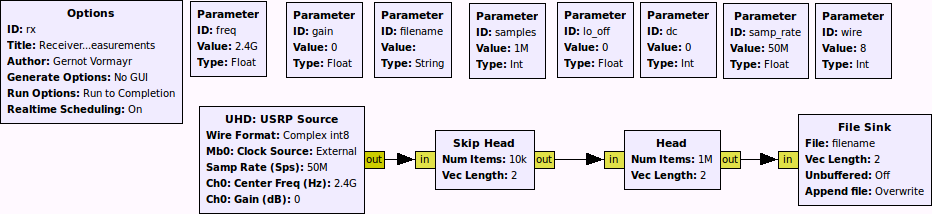
\includegraphics[width=\linewidth]{grc}
    \caption{GNU Radio companion RX flowgraph}
    \label{fig:grc_rx}
\end{figure}
An example flowgraph, which has been used for RX measurements, can be seen in \cref{fig:grc_rx}.
Every flowgraph has an {\ttfamily Options} block, which determines the name of the output module ({\ttfamily ID}),
which GUI to use for the application ({\ttfamily Generate Options}), and some optional runtime options.
{\ttfamily Parameter} blocks can be used for passing values from either a calling flowgraph or as has
been used in this example for passing values via command line arguments. {\ttfamily Type} specifies the
data type, {\ttfamily ID} the name of the command line argument and the name of the generated variable,
and {\ttfamily Value} an optional default. Signal processing blocks have input and/or output ports, that
need to be connected. The flowgraph \cref{fig:grc_rx} creates a gnuradio program, that samples
packets from an USRP source, drops the first \SI{10}{\kilo\samples} ({\ttfamily Skip Head}), and writes
them into the file named {\ttfamily filename} ({\ttfamily File Sink}). {\ttfamily Head} stops processing after the
specified number of samples. Although most of the parameters have numerical values, they actually
reference the parameters on top. GNU Radio Companion displays the default values of the parameters,
if there are any. Compiling this flowgraph creates a python script called {\ttfamily rx.py} which
can now be used directly, or be adapted to requirements, that can not be met by GNU Radio Companion (e.g.
conditionally instantiating flowgraph modules).

\begin{figure}[htbp]
    \centering
    \begin{lstlisting}[basicstyle=\tiny,caption={Generated RX flowgraph module with modifications ({\ttfamily rx\_final.py)}},label=lst:rxfinal.py]
#!/usr/bin/env python
##################################################
# Gnuradio Python Flow Graph
# Title: Receiver for Measurements
# Author: Gernot Vormayr
# Generated: Wed Dec  3 10:00:57 2014
##################################################

from gnuradio import blocks
from gnuradio import eng_notation
from gnuradio import gr
from gnuradio import uhd
from gnuradio.eng_option import eng_option
from gnuradio.filter import firdes
from optparse import OptionParser
import time

class rx(gr.top_block): (*\label{line:classdef}*)
def __init__(self, freq=2.4e9, gain=0, filename="", samples=1000000, lo_off=0, dc=0, samp_rate=50e6, wire=8): (*\label{line:init}*)
        gr.top_block.__init__(self, "Receiver for Measurements")
        if wire == 8: (*\label{line:w81}*)
            otw_format = "sc8"
            bs = gr.sizeof_char*2
        elif wire == 16:
            otw_format = "sc16"
            bs = gr.sizeof_short*2

        ################################################## (*\label{line:blockinst}*)
        # Blocks
        ##################################################
        self.uhd_usrp_source_0 = uhd.usrp_source(
        	device_addr="addr=192.168.10.2",
        	stream_args=uhd.stream_args(
        		cpu_format="sc16",
        		otw_format=otw_format,
        		channels=range(1),
        	),
        )
        self.uhd_usrp_source_0.set_clock_source("external", 0)
        self.uhd_usrp_source_0.set_samp_rate(samp_rate)
        self.uhd_usrp_source_0.set_center_freq(uhd.tune_request(freq, lo_off), 0)
        self.uhd_usrp_source_0.set_gain(gain, 0)
        if dc == 0:
            self.uhd_usrp_source_0.set_auto_dc_offset(False) (*\label{line:dcoff1}*)
	    self.uhd_usrp_source_0.set_dc_offset(0)          (*\label{line:dcoff2}*)
        self.blocks_skiphead_0 = blocks.skiphead(bs, int(samp_rate))
        if wire == 8: (*\label{line:w82}*)
        self.blocks_short_to_char_0 = blocks.short_to_char(2) (*\label{line:short}*)
        self.blocks_head_0 = blocks.head(bs, samples)
        self.blocks_file_sink_0 = blocks.file_sink(bs, filename, False)
        self.blocks_file_sink_0.set_unbuffered(False)

        ################################################## (*\label{line:conninst}*)
        # Connections
        ##################################################
        if wire == 8: (*\label{line:w83}*)
            self.connect((self.uhd_usrp_source_0, 0), (self.blocks_short_to_char_0, 0))
            self.connect((self.blocks_short_to_char_0, 0), (self.blocks_skiphead_0, 0))
        elif wire == 16:
            self.connect((self.uhd_usrp_source_0, 0), (self.blocks_skiphead_0, 0))
        self.connect((self.blocks_skiphead_0, 0), (self.blocks_head_0, 0))
        self.connect((self.blocks_head_0, 0), (self.blocks_file_sink_0, 0))
(*\label{line:setters}*)
if __name__ == '__main__': (*\label{line:main}*)
    parser = OptionParser(option_class=eng_option, usage="%prog: [options]")
    parser.add_option("", "--freq", dest="freq", type="eng_float", default=eng_notation.num_to_str(2.4e9), help="Set freq [default=%default]")
    parser.add_option("", "--gain", dest="gain", type="eng_float", default=eng_notation.num_to_str(0), help="Set gain [default=%default]")
    parser.add_option("", "--filename", dest="filename", type="string", default="", help="Set filename [default=%default]")
    parser.add_option("", "--samples", dest="samples", type="intx", default=1000000, help="Set samples [default=%default]")
    parser.add_option("", "--lo-off", dest="lo_off", type="eng_float", default=eng_notation.num_to_str(0), help="Set lo_off [default=%default]")
    parser.add_option("", "--dc", dest="dc", type="intx", default=0, help="Set dc [default=%default]")
    parser.add_option("", "--samp-rate", dest="samp_rate", type="eng_float", default=eng_notation.num_to_str(50e6), help="Set samp_rate [default=%default]")
    parser.add_option("", "--wire", dest="wire", type="intx", default=8, help="Set wire [default=%default]")
    (options, args) = parser.parse_args()
    if gr.enable_realtime_scheduling() != gr.RT_OK:
        print "Error: failed to enable realtime scheduling."
    tb = rx(freq=options.freq, gain=options.gain, filename=options.filename, samples=options.samples, lo_off=options.lo_off, dc=options.dc, samp_rate=options.samp_rate, wire=options.wire)
    tb.start() (*\label{line:start}*)
    tb.wait() (*\label{line:wait}*)
    \end{lstlisting}
\end{figure}
The generated script follows a predefined structure. An example of a modified python
file can be seen in \cref{lst:rxfinal.py}. Generated versions contain a class
(\cref{line:classdef}) which represents the flowgraph. In the
\lstinline{__init__} function (\cref{line:init}) the whole flowgraph,
starting with the blocks (\cref{line:blockinst}) followed by the connections
(\cref{line:conninst}), is instantiated. Normally GNU Radio Companion would insert
getters and setters for all variables in \cref{line:setters}, but those have been
remove from the script, because those are only needed for graphical user interfaces,
to synchronize the displayed values with the used ones. The last block in the file
represents the main function (\cref{line:main}), which gets executed, when the script
is called directly, instead of importing it into a larger project. This block parses
the arguments handed over to the script, does necessary setup, instantiates
the defined class, starts the processing (\cref{line:start}) asynchronously, and waits for completion
(\cref{line:wait}). \lstinline{tb.stop()} could be used between those two functions to
stop processing early. Additional information on the particular modifications are in
\cref{sec:measgnu}.
%======================================================================
\section{Measurement Setup}
All the measurements and the data processing have been done utilizing the following tools:
\subsection{Mathworks Matlab}
Matlab has been used to automate the measurements, process the raw data, and for
initial visualization of the data. USRP control and data acquisition was planned to
be done in matlab directly with the hardware drivers supplied by Mathworks \cite{matlab_usrp},
which proved futile, because the matlab drivers for
USRP only provide very basic functionality, e.g. support for setting the clock to
external is missing. Another problem was, that matlab was too slow for processing
data at a sample rate of \SI{50}{\mega\samples\per\second}. This led to the approach of
using GNU Radio for communicating with the USRP. Two GNU Radio flowgraphs were
developed and modified, that write the samples to a file in memory or read them
(see \cref{sec:measgnu}). Accompanying Matlab functions were developed that convert
between the binary data and complex Matlab vectors.

Because of no available VISA stack, automation of the meters was done via
SCPI\footnote{Standard Commands for Programmable Instruments} over Ethernet and VXI-11.
To be able to use VXI-11, without a VISA stack, a python library \cite{yamamoto_vxi-11} was
utilized.
\subsection{GNU Radio}
\label{sec:measgnu}
As meantioned in \cref{sec:intgnu}, two communication scripts have been developed with GNU
Radio to write USRP samples to a file, and read samples from a file and send them to the USRP.
Tests showed that right after starting the flowgraph there are phase errors despite a
locked LO, which is checked by the USRP driver. Because of this the flowgraph in \cref{fig:grc_rx}
uses a {\ttfamily Skip Head} module, which skips enough samples.

Since the USRP GNU Radio Companion module has no GUI parameter to turn off DC offset
compensation, the output script was modified by hand. Despite lacking some possibilities
in the interface, it is however possible to do everything within python.
\Cref{line:dcoff1} and \cref{line:dcoff2} in \cref{lst:rxfinal.py} turn off DC offset
compensation by disabling the accumulator and setting the accumulator value to zero 
(see \cref{sec:dsprx}).

Several other additions (\Cref{line:w81,line:w82,line:w83} in \cref{lst:rxfinal.py})
make the flowgraph more dynamic, to support \SI{8}{\bit} and \SI{16}{\bit} mode with
the same python script. In \SI{8}{\bit} mode an additional block in \cref{line:short}
is added to the flowgraph, which converts the short integers from the USRP source to
characters. This is necessary, because the USRP block has a very limited choice of
output data formats.

The transmit script is very similar to the receive script. The only differences are,
that the read file data is repeated in a loop, and an additional functionality
allows for endless streaming, which is cancelled on receiveing a line feed on
standard input.
\subsection{Meters and Measurment Setup}
A Rhode \& Schwarz SMBV 100a, and a Rhode \& Schwarz SMIQ06B were used to generate
signals for RX measurements and as clock reference. Since the SMIQ06B possesses no
Ethernet connectivity, an Agilent E85810 GPIB Etheret bridge provided the necessary
conversion. Power measurements were taken with an Agilent N1914A Power Meter and an
Agilent E9301A Power Sensor. Network parameters and power measurements of specific
spectrum ranges were done with a Rhode \& Schwarz ZVL. In order not to interfere
with the high data rate connection needed by USRP, it used a dedicated network interface.

The TX measurement data was corrected with the S-Parameters of the cable and
attenuators, and the RX measurements by measuring the signal power arriving at
the USRP by replacing the USRP with the power meter.

\Cref{sec:rfsetup,sec:ifsetup,sec:imsetup} describe each setup in more detail.

\subsubsection{RF Frequency Response}
\label{sec:rfsetup}
\begin{figure}[htb]
    \begin{subfigure}[t]{.5\linewidth}
        \centering
        \scalebox{0.8}{
        \begin{tikzpicture}
            \matrix (m) [matrix of nodes,
                row sep=1cm,
                column sep=1cm,
                ampersand replacement=\&,
                nodes={draw,
                    line width=1pt,
                    anchor=center, 
                    text centered,
                    minimum width=1.5cm,
                    minimum height=8mm
                }]
            {
                |[rounded corners]| USRP \& \SI{6}{\deci\bel} attn \& |[rounded corners]| SMBV \\
                |[rounded corners]| \begin{tabular}{l}PC \\ Matlab\end{tabular} \& \\
            };
            \draw[dashed] (m-2-1) -- node [pos=0.25,auto] {eth0} (m-1-1);
            \draw[rounded corners,dashed] (m-2-1)  -| node [pos=0.05,auto] {eth1} (m-1-3);
            \draw[double,thick] (m-1-1) -- node [pos=0.3,auto] {RX} (m-1-2) -- (m-1-3);
        \end{tikzpicture}
        }
        \caption{RX}
    \end{subfigure}
    \begin{subfigure}[t]{.5\linewidth}
        \centering
        \scalebox{0.8}{
        \begin{tikzpicture}
            \matrix (m) [matrix of nodes,
                row sep=1cm,
                column sep=1cm,
                ampersand replacement=\&,
                nodes={draw,
                    line width=1pt,
                    anchor=center, 
                    text centered,
                    minimum width=1.5cm,
                    minimum height=8mm
                }]
            {
                |[rounded corners]| USRP \& \SI{16}{\deci\bel} attn \& |[rounded corners]| Power Meter \\
                |[rounded corners]| \begin{tabular}{l}PC \\ Matlab\end{tabular} \& \\
            };
            \draw[dashed] (m-2-1) -- node [pos=0.25,auto] {eth0} (m-1-1);
            \draw[rounded corners,dashed] (m-2-1)  -| node [pos=0.05,auto] {eth1} (m-1-3);
            \draw[double,thick] (m-1-1) -- node [pos=0.3,auto] {TX} (m-1-2) -- (m-1-3);
        \end{tikzpicture}
        }
        \caption{TX}
    \end{subfigure}
    \caption{RF frequency response measurement setup}
    \label{fig:rfsetup}
\end{figure}
\Cref{fig:rfsetup} depicts the basic measurement setup.

Since the power head can only measure signals between \SI{-60}{\deci\belm} and
\SI{20}{\deci\belm} a \SI{6}{\deci\bel} and a \SI{10}{\deci\bel} attenuator were used,
to bring down the signal to acceptable levels. Since the USRP shows high DC levels,
caused by the mixer used, the RF frequency response has been measured with an offset
of 1 MHz. DC offset correction is not an option, since this removes DC completely.

\subsubsection{IF Frequency Response}
\label{sec:ifsetup}
\begin{figure}[htb]
    \begin{subfigure}[t]{.5\linewidth}
        \centering
        \scalebox{0.8}{
        \begin{tikzpicture}
            \matrix (m) [matrix of nodes,
                row sep=1cm,
                column sep=1cm,
                ampersand replacement=\&,
                nodes={draw,
                    line width=1pt,
                    anchor=center, 
                    text centered,
                    minimum width=1.5cm,
                    minimum height=8mm
                }]
            {
                |[rounded corners]| USRP \& |[rounded corners]| SMIQ \\
                |[rounded corners]| \begin{tabular}{l}PC \\ Matlab\end{tabular} \& |[rounded corners]| GPIB bridge \\
            };
            \draw[dashed] (m-2-1) -- node [pos=0.25,auto] {eth0} (m-1-1);
            \draw[rounded corners,dashed] (m-2-1)  -- node [pos=0.45,auto] {eth1} (m-2-2);
            \draw[rounded corners,dashdotted] (m-2-2) -- (m-1-2);
            \draw[double,thick] (m-1-1) -- node [pos=0.3,auto] {RX} (m-1-2);
        \end{tikzpicture}
        }
        \caption{RX}
    \end{subfigure}
    \begin{subfigure}[t]{.5\linewidth}
        \centering
        \scalebox{0.8}{
        \begin{tikzpicture}
            \matrix (m) [matrix of nodes,
                row sep=1cm,
                column sep=1cm,
                ampersand replacement=\&,
                nodes={draw,
                    line width=1pt,
                    anchor=center, 
                    text centered,
                    minimum width=1.5cm,
                    minimum height=8mm
                }]
            {
                |[rounded corners]| USRP \& \SI{16}{\deci\bel} attn \& |[rounded corners]| ZVL \\
                |[rounded corners]| \begin{tabular}{l}PC \\ Matlab\end{tabular} \& \\
            };
            \draw[dashed] (m-2-1) -- node [pos=0.25,auto] {eth0} (m-1-1);
            \draw[rounded corners,dashed] (m-2-1)  -| node [pos=0.05,auto] {eth1} (m-1-3);
            \draw[double,thick] (m-1-1) -- node [pos=0.3,auto] {TX} (m-1-2) -- (m-1-3);
        \end{tikzpicture}
        }
        \caption{TX}
    \end{subfigure}
    \caption{IF frequency response measurement setup}
    \label{fig:ifsetup}
\end{figure}
Because of availability issues, the SMIQ was used for the setup in \cref{fig:ifsetup}.
This setup used an attenuator, for the same reasons mentioned in \ref{sec:rfsetup}.

For TX measurement the ZVL was used, unlike in \cref{sec:rfsetup}L, to be able to isolate
only the intended frequency.

\subsubsection{Intermodulation Properties}
\label{sec:imsetup}
\begin{figure}[htb]
    \begin{subfigure}[t]{.5\linewidth}
        \centering
        \scalebox{0.8}{
        \begin{tikzpicture}
            \matrix (m) [matrix of nodes,
                row sep=1cm,
                column sep=1cm,
                ampersand replacement=\&,
                nodes={draw,
                    line width=1pt,
                    anchor=center, 
                    text centered,
                    minimum width=1.5cm,
                    minimum height=8mm
                }]
            {
                |[rounded corners]| USRP \& |[shape=circle]| splitter \& \SI{10}{\deci\bel} attn \\
                \& \SI{10}{\deci\bel} attn \& DC Block \\
                     \& DC Block \& |[rounded corners]| SMIQ\\
                     \& |[rounded corners]| SMBV \& |[rounded corners]| GPIB bridge \\
                |[rounded corners]| \begin{tabular}{l}PC \\ Matlab\end{tabular} \& \\
            };
            \draw[double,thick] (m-1-1) -- node [pos=0.3,auto] {RX} (m-1-2) -- (m-1-3) -- (m-2-3) -- (m-3-3);
            \draw[double,thick] (m-1-2) -- (m-2-2) -- (m-3-2) -- (m-4-2);
            \draw[dashed] (m-5-1) -- node [pos=0.05,auto] {eth0} (m-1-1);
            \draw[rounded corners,dashed] (m-5-1)  -| node [pos=0.12,auto] {eth1} (m-4-2);
            \draw[rounded corners,dashed] (m-5-1)  -| (m-4-3);
            \draw[rounded corners,dashdotted] (m-4-3) -- (m-3-3);
        \end{tikzpicture}
        }
        \caption{RX}
    \end{subfigure}
    \begin{subfigure}[t]{.5\linewidth}
        \centering
        \scalebox{0.8}{
        \begin{tikzpicture}
            \matrix (m) [matrix of nodes,
                row sep=1cm,
                column sep=1cm,
                ampersand replacement=\&,
                nodes={draw,
                    line width=1pt,
                    anchor=center, 
                    text centered,
                    minimum width=1.5cm,
                    minimum height=8mm
                }]
            {
                |[rounded corners]| USRP \& \SI{16}{\deci\bel} attn \& |[rounded corners]| ZVL \\
                |[rounded corners]| \begin{tabular}{l}PC \\ Matlab\end{tabular} \& \\
            };
            \draw[dashed] (m-2-1) -- node [pos=0.25,auto] {eth0} (m-1-1);
            \draw[rounded corners,dashed] (m-2-1)  -| node [pos=0.05,auto] {eth1} (m-1-3);
            \draw[double,thick] (m-1-1) -- node [pos=0.3,auto] {TX} (m-1-2) -- (m-1-3);
        \end{tikzpicture}
        }
        \caption{TX}
    \end{subfigure}
    \caption{Intermodulation properties measurement setup}
    \label{fig:imsetup}
\end{figure}
TX measurement used the same setup as described in \cref{sec:ifsetup}. Multiple
measurements with random phases were taken.

At first for RX a similar measurement setup as in \cref{sec:rfsetup} was attempted,
but it was not possible to generate a signal free of intermodulation products with
the SMBV. With the ZVL, it was verified, that those products are caused by the
SMBV. This led to the setup in \cref{fig:imsetup}. This setup utilized a Mini-Circuits
ZFRSC-183+ power splitter/combiner. Since this is a resistive power splitter, it has
very poor isolation\cite{pwrsplit}. In order to prevent the signal generators from
distorting the output because of this coupling the \SI{10}{\deci\bel} attenuator
and the DC block were used.
%======================================================================
\clearpage
\section{Measurement Results}
All the circuit designations in the following sections refer to \cref{fig:usrp}.
\subsection{RF Frequency Response}
\subsubsection{RX}
\label{sec:rfrx}
\begin{figure}[htb]
    \centering
\begin{tikzpicture}
    \begin{axis}[
        xlabel={gain},
        ylabel={power},
        x unit={\deci\bel},
        y unit={\deci\belm},
        minor tick num = 1
        ]
        \addplot[mark = +,red] table {data/rf/rx/8/dbm_400};
        \addlegendentry{\SI{400}{MHz}}
        \addplot[mark = x,green] table {data/rf/rx/8/dbm_2400};
        \addlegendentry{\SI{2.4}{GHz}}
        \addplot[mark = asterisk,blue] table {data/rf/rx/8/dbm_4400};
        \addlegendentry{\SI{4.4}{GHz}}
    \end{axis}
\end{tikzpicture}
    \caption{Input power needed for \SI{0}{\deci\belfs}}
    \label{fig:inputfscrf}
\end{figure}
\begin{figure}[htb]
    \centering
\begin{tikzpicture}
    \begin{axis}[
        legend pos=north west,
        legend columns=2,
        ylabel={gain},
        xlabel={frequency},
        y unit={\deci\bel},
        x unit={\hertz},
        change x base,
        x SI prefix=giga,
        width=\linewidth,
        height=7cm,
        minor tick num = 1
        ]
        \addplot[red] table {data/rf/rx/8/f_0};
        \addlegendentry{\SI{0}{dBm}}
        \addplot[green] table {data/rf/rx/8/f_15};
        \addlegendentry{\SI{15}{dBm}}
        \addplot[blue] table {data/rf/rx/8/f_30};
        \addlegendentry{\SI{30}{dBm}}
    \end{axis}
\end{tikzpicture}
    \caption{Gain needed for \SI{0}{\deci\belfs}}
    \label{fig:gainfscrf}
\end{figure}
Measurement results are provided in \cref{fig:inputfscrf,fig:gainfscrf}.
\Cref{fig:inputfscrf} reflects the maximum gain setting of \SI{31.5}{\deci\bel}.
The loss in gain over the frequency range in \cref{fig:gainfscrf} is mainly caused
by LNA1 and LNA2 \cite{rxlna} and the ripples by the DEMOD \cite{demod}.

\subsubsection{TX}
\label{sec:rftx}
\begin{figure}[htb]
    \centering
\begin{tikzpicture}
    \begin{axis}[
        legend pos = south west,
        legend columns = -1,
        ylabel={power},
        xlabel={frequency},
        y unit={\deci\belm},
        x unit={\hertz},
        change x base,
        x SI prefix=giga,
        width=\linewidth,
        height=7cm,
        minor tick num = 1,
        ymin = -25
        ]
        \addplot[red] table {data/rf/tx/0.8/0.0};
        \addplot[green] table {data/rf/tx/0.8/10.0};
        \addplot[blue] table {data/rf/tx/0.8/20.0};
        \addplot[black] table {data/rf/tx/0.8/30.0};
        \addplot[violet] table {data/rf/tx/0.8/31.5};
        \legend{\SI{0}{dB},\SI{10}{dB},\SI{20}{dB},\SI{30}{dB},\SI{31.5}{dB}}
    \end{axis}
\end{tikzpicture}
\caption{Output power, \SI{-1.94}{\deci\belfs}}
    \label{fig:outputrf08}
\end{figure}
\begin{figure}[htb]
    \centering
\begin{tikzpicture}
    \begin{axis}[
        legend pos = south west,
        legend columns = -1,
        ylabel={power},
        xlabel={frequency},
        y unit={\deci\belm},
        x unit={\hertz},
        change x base,
        x SI prefix=giga,
        width=\linewidth,
        height=7cm,
        minor tick num = 1,
        ymin = -25
        ]
        \addplot[red] table {data/rf/tx/1.0/0.0};
        \addplot[green] table {data/rf/tx/1.0/10.0};
        \addplot[blue] table {data/rf/tx/1.0/20.0};
        \addplot[black] table {data/rf/tx/1.0/30.0};
        \addplot[violet] table {data/rf/tx/1.0/31.5};
        \legend{\SI{0}{dB},\SI{10}{dB},\SI{20}{dB},\SI{30}{dB},\SI{31.5}{dB}}
    \end{axis}
\end{tikzpicture}
    \caption{Output power, \SI{0}{\deci\belfs}}
    \label{fig:outputrf1}
\end{figure}
Measurements were done at \SI{0}{\deci\belfs} and \SI{-1.94}{\deci\belfs}. The
results can be seen in \cref{fig:outputrf08,fig:outputrf1}. AMP2 \cite{amp2} and AMP3
\cite{amp3} are the main cause for the loss in gain over the frequency range.

\subsection{IF Frequency Response}
\subsubsection{RX}
\label{sec:ifrx}
\begin{figure}[htb]
    \centering
\begin{tikzpicture}
    \begin{axis}[
        ylabel={IF frequency},
        xlabel={RF frequency},
        zlabel={input power},
        xlabel style={sloped},
        ylabel style={sloped},
        x unit={\hertz},
        change x base,
        x SI prefix=giga,
        y unit={\hertz},
        change y base,
        y SI prefix=mega,
        z unit={\deci\belm},
        z dir=reverse,
        width=\linewidth,
        height=7cm,
        minor tick num = 1,
        ]
        \addplot3[surf,mesh/cols=41] table {data/if/rx/mesh16_15.0};
    \end{axis}
\end{tikzpicture}
    \caption{Input power needed for \SI{0}{\deci\belfs}, \SI{16}{\bit}, \SI{15}{\deci\bel} gain, \SI{25}{\mega\samples\per\second}}
    \label{fig:rfifrx16}
\end{figure}
\begin{figure}[htb]
    \centering
\begin{tikzpicture}
    \begin{axis}[
        legend style={at={(0.5,0.97)},anchor=north},
        xlabel={IF frequency},
        ylabel={input power},
        x unit={\hertz},
        change x base,
        x SI prefix=mega,
        y unit={\deci\belm},
        width=\linewidth,
        height=5cm,
        minor tick num = 1,
        ]
        \addplot[red] table {data/if/rx/16_2000_15.0};
        \addlegendentry{\SI{16}{\bit}}
        \addplot[green] table {data/if/rx/825_2000_15.0};
        \addlegendentry{\SI{8}{\bit}}
    \end{axis}
\end{tikzpicture}
    \caption{Input power needed for \SI{0}{\deci\belfs}, \SI{15}{\deci\bel} gain, RF frequency \SI{2}{\giga\hertz}, \SI{25}{\mega\samples\per\second}}
    \label{fig:ifrx25}
\end{figure}
\begin{figure}[htb]
    \centering
\begin{tikzpicture}
    \begin{axis}[
        legend style={at={(0.5,0.97)},anchor=north},
        xlabel={IF frequency},
        ylabel={input power},
        x unit={\hertz},
        change x base,
        x SI prefix=mega,
        y unit={\deci\belm},
        width=\linewidth,
        height=5cm,
        minor tick num = 1,
        ]
        \addplot[red] table {data/if/rx/8_2000_15.0};
        \addlegendentry{\SI{16}{\bit}}
    \end{axis}
\end{tikzpicture}
    \caption{Input power needed for \SI{0}{\deci\belfs}, \SI{15}{\deci\bel} gain, RF frequency \SI{2}{\giga\hertz}, \SI{25}{\mega\samples\per\second}}
    \label{fig:ifrx50}
\end{figure}
An overview of the measurement results can be seen in \cref{fig:rfifrx16}. The slope and ripple
in the RF frequency direction is uniformly distributed along the IF frequency axis.
These results and different gain settings, which can be found in the measurement data \ref{sec:sources},
reproduce the same result as in \cref{sec:rfrx}. Since these measurements were taken without DC offset
compensation, there is a small peak at \SI{0}{\mega\hertz}, which is caused by DEMOD \cite{demod}.

In \ref{fig:ifrx50} the effect of the \SI{20}{\mega\hertz} filter mentioned in \cref{sec:usrp} is
observable.

\subsubsection{TX}
\label{sec:iftx}
\begin{figure}[htb]
    \centering
\begin{tikzpicture}
    \begin{axis}[
        ylabel={IF frequency},
        xlabel={RF frequency},
        zlabel={output power},
        xlabel style={sloped},
        ylabel style={sloped},
        x unit={\hertz},
        change x base,
        x SI prefix=giga,
        y unit={\hertz},
        change y base,
        y SI prefix=mega,
        z unit={\deci\belm},
        width=\linewidth,
        height=7cm,
        minor tick num = 1,
        ]
        \addplot3[surf,mesh/cols=41] table {data/if/tx/mesh16_15.0};
    \end{axis}
\end{tikzpicture}
    \caption{Output power \SI{-3.10}{\deci\belfs}, \SI{16}{\bit}, \SI{15}{\deci\bel} gain, \SI{25}{\mega\samples\per\second}}
    \label{fig:rfiftx16}
\end{figure}
\begin{figure}[htb]
    \centering
\begin{tikzpicture}
    \begin{axis}[
        xlabel={IF frequency},
        ylabel={output power},
        x unit={\hertz},
        change x base,
        x SI prefix=mega,
        y unit={\deci\belm},
        width=\linewidth,
        height=5cm,
        minor tick num = 1,
        ]
        \addplot[red] table {data/if/tx/16_2000_15.0};
    \end{axis}
\end{tikzpicture}
    \caption{Output power \SI{-3.10}{\deci\belfs}, \SI{15}{\deci\bel} gain, RF frequency \SI{2}{\giga\hertz}, \SI{25}{\mega\samples\per\second}, \SI{16}{\bit}}
    \label{fig:iftx}
\end{figure}
\begin{figure}[htb]
    \centering
\begin{tikzpicture}
    \begin{axis}[
        xlabel={IF frequency},
        ylabel={output power},
        x unit={\hertz},
        change x base,
        x SI prefix=mega,
        y unit={\deci\belm},
        width=\linewidth,
        height=5cm,
        minor tick num = 1,
        ]
        \addplot[red] table {data/if/tx/8_2000_15.0};
    \end{axis}
\end{tikzpicture}
    \caption{Output power \SI{-3.10}{\deci\belfs}, \SI{15}{\deci\bel} gain, RF frequency \SI{2}{\giga\hertz}, \SI{50}{\mega\samples\per\second}, \SI{8}{\bit}}
    \label{fig:iftx50}
\end{figure}
The overview in \cref{fig:rfiftx16} has the same slope and ripple
in the RF frequency direction as \cref{sec:rftx}. Both are uniformly
distributed along the IF frequency axis. \cref{fig:iftx} features only the \SI{16}{\bit}
measurement, because the \SI{8}{\bit} measurement produced the same result.

In \ref{fig:iftx50} the effect of the \SI{20}{\mega\hertz} filter mentioned in \cref{sec:usrp} is
observable.

\clearpage
\subsection{Intermodulation Properties}
\subsubsection{RX}
\begin{figure}[htb]
    \centering
\begin{tikzpicture}
    \begin{axis}[
        legend pos = south east,
        ylabel={output power},
        xlabel={input power},
        y unit={\deci\belfs},
        x unit={\deci\belm},
        width=\linewidth,
        height=6cm,
        minor tick num = 1,
        ]
        \addplot[only marks, mark = +] table {data/ip3/rx/la};
        \addplot[only marks, mark = x] table {data/ip3/rx/im3};
        \addplot[only marks, mark = asterisk] table {data/ip3/rx/pim3};
        \addplot[domain = -93:-35, samples = 201,green] {1*x+33.0765};
        \addplot[domain = -93:-35, samples = 201,red] {3*x+111.2541};
        \legend{$out$,$IM_3$,$IP_3$}
    \end{axis}
\end{tikzpicture}
    \caption{RX IP3}
    \label{fig:rxip3}
\end{figure}
Stepping the gain did not result in noticeable intermodulation products.
Because of this the measurement was done at a fixed gain setting of
\SI{31.5}{\deci\bel}. This also means that the intermodulation products
in \cref{fig:rxip3} are caused by the DAC.
\subsubsection{TX}
\begin{figure}[htb]
    \centering
\begin{tikzpicture}
    \begin{axis}[
        legend pos = south east,
        ylabel={output power},
        xlabel={input power},
        x unit={\deci\belfs},
        y unit={\deci\belm},
        width=\linewidth,
        height=6cm,
        minor tick num = 1,
        ]
        \addplot[only marks, mark = +] table {data/ip3/tx/la};
        \addplot[only marks, mark = x] table {data/ip3/tx/im3};
        \addplot[only marks, mark = asterisk] table {data/ip3/tx/pim3};
        \addplot[domain = -27:17, samples = 201,green] {1*x-4.2330};
        \addplot[domain = -27:17, samples = 201,red] {3*x-33.6197};
        \legend{$out$,$IM_3$,$IP_3$}
    \end{axis}
\end{tikzpicture}
    \caption{TX IP3}
    \label{fig:txip3}
\end{figure}
Stepping the gain or changing the settings on the ZVL did not result
in intermodulation products. Because of this the measurement was done
at a fixed gain setting of \SI{20}{\deci\bel}. This also means that
the intermodulation products in \cref{fig:txip3} are caused by the ADC.

%======================================================================
\clearpage
\begin{appendix}
\section{Measurement results and Source Code}
\label{sec:sources}
All the raw data, processed results and sources can be found at
\url{https://github.com/notti/usrp_measurements}.
\section*{Copyright}
This work is licensed under the Creative Commons Attribution 4.0 International
License. To view a copy of this license, visit
\url{http://creativecommons.org/licenses/by/4.0/} or send a letter to Creative
Commons, 444 Castro Street, Suite 900, Mountain View, California, 94041, USA.

\printglossary[type=\acronymtype]

\listoffigures

\bibliographystyle{IEEEtran}
\bibliography{IEEEabrv,literature}
\end{appendix}

\end{document}
